\documentclass[11pt,landscape,a4paper]{article}
\newcommand\hmmax{0}
\newcommand\bmmax{0}
\usepackage[utf8]{inputenc}
\usepackage[ngerman]{babel}
\usepackage{amsmath}
\usepackage{amsfonts}
\usepackage{bbm}
\usepackage{bm}
\usepackage[x11names]{xcolor}
\usepackage{todonotes}

\usepackage{tikz}
\usetikzlibrary{shapes,positioning,arrows,fit,calc,graphs,graphs.standard}

%fonts:
%\usepackage[nosf]{kpfonts}
\usepackage[t1]{sourcesanspro}


%\usepackage[lf]{MyriadPro}
%\usepackage[lf,minionint]{MinionPro}
\usepackage{multicol}
\usepackage{wrapfig}
\usepackage[landscape,paper=a4paper,margin=0.25cm]{geometry}
% \usepackage[top=0mm,bottom=4mm,left=0mm,right=1mm]{geometry}
% \usepackage[framemethod=tikz]{mdframed}
%\usepackage{microtype}
%\usepackage{mathptmx}
%\usepackage{cm}
\usepackage{amssymb}
\usepackage{dsfont}

% Custom for mapto with text on top
\usepackage{stmaryrd}

\usepackage{paralist}
\usepackage[framemethod=tikz]{mdframed}
%Commands
\newcommand{\y}{\mathbf{y}}
\newcommand{\x}{\mathbf{x}}
\newcommand{\z}{\mathbf{z}}
\newcommand{\w}{\mathbf{w}}
\newcommand{\Z}{\mathcal{Z}}
\newcommand{\X}{\mathbf{X}}
\newcommand{\Y}{\mathbf{Y}}
\newcommand{\I}{\mathbf{I}}
\newcommand{\B}{\mathbf{B}}
\newcommand{\N}{\mathcal{N}}
\newcommand{\E}{\mathbb{E}}
\newcommand{\Prob}{\mathrm{\textbf{P}}}
\newcommand{\V}{\mathbb{V}}
\newcommand{\C}{\mathbb{C}}
\newcommand{\R}[0]{\mathbb{R}}
\DeclareMathOperator*{\argmin}{arg\,min}
\DeclareMathOperator*{\argmax}{arg\,max}

%Maps to with text on top%
\makeatletter
\newcommand{\xMapsto}[2][]{\ext@arrow 0599{\Mapstofill@}{#1}{#2}}
\def\Mapstofill@{\arrowfill@{\Mapstochar\Relbar}\Relbar\Rightarrow}
\makeatother

\endinput


\thinmuskip=1mu
\medmuskip=1mu %plus 2mu minus 4mu
\thickmuskip=1mu
\let\bar\overline

%\definecolor{mygrey}{cmyk}{0,0,0,0.8}
\definecolor{mathColor}{cmyk}{0,0,0,0.9}

\definecolor{sectionColor}{HTML}{4B0082}
\definecolor{subsectionColor}{HTML}{3364FF}

\DeclareMathOperator{\di}{d\!}
\DeclareMathAlphabet{\mathcal}{OMS}{cmsy}{}{n}

\pgfdeclarelayer{background}
\pgfsetlayers{background,main}

\everymath\expandafter{\the\everymath \color{mathColor}}
\everydisplay\expandafter{\the\everydisplay \color{mathColor}}

\renewcommand{\baselinestretch}{.75}
\pagestyle{empty}


\makeatletter
\renewcommand{\section}{\@startsection{section}{1}{0mm}%
                                {.2ex}%
                                {.2ex}%x
                                {\color{sectionColor}\sffamily\small\bfseries}}
%Firebrick1
\renewcommand{\subsection}{\@startsection{subsection}{1}{0mm}%
                                {.2ex}%
                                {.2ex}%x
                                {\color{subsectionColor}\sffamily\bfseries}}
\renewcommand{\subsubsection}{\@startsection{subsubsection}{1}{0mm}%
                                {0ex}%
                                {0.1ex}%x
                                {\sffamily\bfseries}}
% \usepackage{titlesec}
% \titlespacing*{\subsubsection}{0pt}{-2pt}{-6pt}


\makeatother
\setlength{\parindent}{0pt}
\setlength{\columnsep}{5pt}

\begin{document}
\small
\begin{multicols*}{4}
\fontdimen2\font=0.3ex
\subsection*{Probabilities}

$\E_{Y|X}[Y]=\E_{Y}[Y|X]$

$\E_{X,Y}[f(X,Y)]=\E_{X}\E_{Y|X}[f(X,Y)|X]$

$\E_{Y|X}[f(X,Y)|X]{=}\int_\mathbb{R}f(X,y)\Prob(y|X)\di y$

$\C(\X,\Y)=\E[(\X-\E[\X])(\Y-\E[\Y])] = \E[\X\Y^T]-\E[\X]\E[\Y]^T$

$\C(\mathbf{a}\X,\mathbf{b}\Y)=\mathbf{a}\C(\X,\Y)\mathbf{b}^T$

$P(A|B) = \frac{P(B|A) \cdot P(A)}{P(B)}$; $p(Z|X,\theta) = \frac{p(X,Z|\theta)}{p(X|\theta)}$

Vec. Var: $\mathbb V[\mathbf x]=\mathbb E[\mathbf x\mathbf x^T]-\mathbb E[\mathbf x]\mathbb E[\mathbf x]^T=\mathbb E[\mathbf w\mathbf w^T]-\mathbb E[\mathbf w]\mathbb E[\mathbf w]^T$

$P(x,y) = P(y|x) \cdot  P(x) = P(x|y) \cdot P(y)$
$P(x)=\sum_i P(x|y=i)P(y=i)$

\subsection*{Distributions}
$\mathcal{N}(x|\mu, \sigma^2)=\frac{\exp(-\frac{1}{2}\frac{(x-\mu)^2}{\sigma^2})}{\sqrt{2\pi\sigma^2}}$;\\
$\N(x|\mu, \Sigma)= \frac{\exp(-\frac{1}{2}(\mathbf{x}-\mu)^T\Sigma^{-1}(\mathbf{x}-\mu))}{(2\pi)^{D/2}|\Sigma|^{1/2}}$;\\
Emp.: $\hat{\Sigma} = \frac{1}{n}\sum_{i=1}^n x_i x_i^T$ (need centered data)\\
$\E[X^2]= \Sigma+ \mu\mu^T, \E[\hat{\sigma}^2]=\frac{n-1}{n}\sigma^2 $\\
$\mathrm{Exp}(x|\lambda){=}\lambda e^{-\lambda x}; \, \frac{1}{\lambda}; \, \frac{1}{\lambda^2}$\\
$\mathrm{Ber}(x|\theta){=}\theta^x (1{-}\theta)^{(1-x)}$;$ \, \theta$;$ \, \theta(1-\theta)$\\
$\mathrm{Bin}(n|\theta)=\binom{n}{x}\theta^{x}(1-\theta)^{(n-x)}$;$n\uparrow$;$n\uparrow$

\subsection*{Norms}
Frobenius norm: $\|\mathbf A\|_F = \left(\sum_{i,j}A_{i,j}^2\right)^\frac{1}{2}$

\subsection*{Jensen}
$\phi(\E)\leq \E[\phi]$; $\phi$ convex (reversed if concave:)$\E[\min]\leq \min\E$;$\E[\log]\leq\log\E$
\subsection*{Convex, smooth $f(x)$}
$f''(x) > 0 \Leftrightarrow x_1,x_2 \in \mathbb{R}, \lambda \in [0,1]:
f(\lambda x_1 + (1-\lambda) x_2) \leq \lambda f(x_1) + (1-\lambda) f(x_2)$\\
strong: 
$f(x+y)\geq f(x)+\nabla f(x)\cdot y+\frac{\mu}{2}\| y\|$\\
L-smooth: $\| \nabla f(x)-\nabla f(x+y)\|\leq L\|y\|$, $f\in C^2: f(x+y)\leq f(x)+\nabla f(x)\cdot y+\frac{L}{2}\| y\|^2$;
$\mu \preceq \nabla^2f \preceq L$


\subsection*{Pos semi-definite mat $M \in \mathbb{R}^{n\times n}$}
$\forall x \in \mathbb{R}^n: x^TMx \geq 0 \Leftrightarrow$ eigenvalues $\lambda_i\geq 0$
\subsection*{Completing squares}
$x^{\mathrm {T} }Ax+x^{\mathrm {T} }b+c=(x-h)^{\mathrm {T} }A(x-h)+k$ \\
$A=A^{\mathrm {T} }:\quad h=-{\frac {1}{2}}A^{-1}b,\quad k=c-{\frac {1}{4}}b^{\mathrm {T} }A^{-1}b$\\
$h=-(A+A^{\mathrm {T} })^{-1}b,\quad k=c-h^{\mathrm {T} }Ah=c-b^{\mathrm {T} }(A+A^{\mathrm {T} })^{-1}A(A+A^{\mathrm {T} })^{-1}b$\\
$\mathbf{x}^T\mathbf{A}\mathbf{x}-2\mathbf{b}^T\mathbf{x} = (\mathbf{x}-\mathbf{A}^{-1}\mathbf{b})^T\mathbf{A}(\mathbf{x}-\mathbf{A}^{-1}\mathbf{b})-\mathbf{b}^T\mathbf{A}^{-1}\mathbf{b}$;\\
$ax^{2}+bx+c=a(x+\frac{b}{2a})^{2}+c-\frac{b^2}{4a}$

\subsection*{Derivatives}

$\frac{\text{d}}{\text{d}\mathbf x}\mathbf x^T\mathbf B=\mathbf B = \frac{\text{d}}{\text{d}\mathbf x}\mathbf B\mathbf x$

$\frac{\text{d}}{\text{d}\mathbf x}\mathbf x^T\mathbf b=\mathbf b$

$\frac{\text{d}}{\text{d}\mathbf x}\mathbf x^T\mathbf x=2\mathbf x$

$\frac{\text{d}}{\text{d}\mathbf x}\mathbf x^T\mathbf B \mathbf x=2\mathbf B\mathbf x$

$\frac{\text{d}}{\text{d}\mathbf B}\mathbf x^T\mathbf B \mathbf x=\mathbf x^T\mathbf x$


$\nabla_v f(w)=\nablaf(w)^T v=\lim_{\lambda \rightarrow 0}\frac{f(w+\lambda v)-f(w)}{\lambda}$

$\nabla_\x\log(1+\exp(-\alpha x))=\frac{-\alpha}{1+\exp(\alpha x)}$
$\frac{\partial}{\partial \mathbf{x}}(\mathbf{x}^\top \mathbf{A}\mathbf{x}) = (\mathbf{A}^\top + \mathbf{A})\mathbf{x} (= 2\mathbf{A}\x$ if symm) \quad\\
$\frac{\partial}{\partial \mathbf{x}}(\mathbf{b}^\top \mathbf{A}\mathbf{x}) = \mathbf{A}^\top \mathbf{b}$ \quad
$\frac{\partial}{\partial \mathbf{X}}(\mathbf{c}^\top \mathbf{X} \mathbf{b}) = \mathbf{c}\mathbf{b}^\top$ \quad
$\frac{\partial}{\partial \mathbf{x}}(\| \mathbf{x}-\mathbf{b} \|_2) = \frac{\mathbf{x}-\mathbf{b}}{\|\mathbf{x}-\mathbf{b}\|_2}$

$\frac{\partial}{\partial \mathbf{x}}(\| \mathbf{x}-\mathbf{b} \|_2^2) = 2(\mathbf x -\mathbf b)$

$\frac{\partial}{\partial \mathbf{x}}(\|\mathbf{x}\|^2_2) = \frac{\partial}{\partial \mathbf{x}} (\mathbf{x}^\top \mathbf{x}) = 2\mathbf{x}$ \quad
\\$\frac{\partial}{\partial \mathbf{X}}(\|\mathbf{X}\|_F^2) = 2\mathbf{X}$  \quad \quad
$\frac{\partial}{\partial \mathbf{x}}||\mathbf{x}||_1 = \frac{\mathbf{x}}{|\mathbf{x}|}$ \\
$\frac{\partial}{\partial \mathbf{x}}(\|\mathbf{Ax - b}\|_2^2) = \mathbf{2(A^\top Ax-A^\top b)}$ \quad
$\frac{\partial}{\partial \mathbf{X}}(|\mathbf{X}|) = |\mathbf{X}|\cdot \mathbf{X}^{-1}$ $\quad |X| = 1 / |X^{-1}|$\\
$\frac{\partial}{\partial x}(\mathbf{Y}^{-1}) = -\mathbf{Y}^{-1} \frac{\partial\mathbf{Y}}{\partial x} \mathbf{Y}^{-1}$

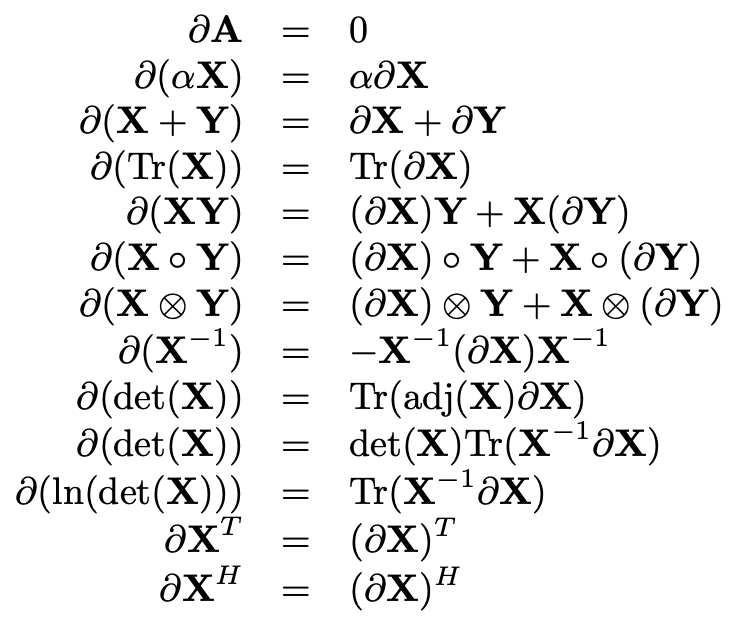
\includegraphics[width=.7\columnwidth]{src/matrix_deriv.png}

\subsection*{Matrices}

Cauchy-Schwarz: $\mathbf a^\top\mathbf b \leq \|\mathbf a\|_2\|\mathbf b\|_2$

Norms: $\mathbf w^\top\mathbf w=\|\mathbf w\|_2^2$, $\mathbf w^\top\text{sgn}(\mathbf w)=\sum_i |x_i|=\|\mathbf w \|_1$

Traces: $\text{Tr}(A+B)=\text{Tr}(A)+\text{Tr}(B)$, $\text{Tr}(AB)=\text{Tr}(BA)$, $\mathbf{a}^T \mathbf a = \text{Tr}(\mathbf{aa}^T)$, $\mathbf x^T\mathbf M\mathbf x=\text{Tr}(\mathbf x^T\mathbf M\mathbf x)$, $\mathbf x^T\mathbf y = \text{Tr}(\mathbf{yx}^T)$, if $\mathbf A$ s.p.d then $\text{Tr}(\mathbf A)\geq 0$.

Vector projection $\mathbf a$ to $\mathbf b$: $\frac{\mathbf a^\top \mathbf b}{\|\mathbf b\|^2}\mathbf b$

\iffalse
\subsection*{Parametric vs. Nonparametric}
\textbf{Parametric}: have finite set of parameters. 
e.g. linear regression, linear perceptron\\
\textbf{Nonparametric}: grow in complexity with the size of the data, more expressive.
e.g. k-NN
\fi
\section*{Chapter 2: Connectionism}
%\section*{Probabilities}
%\subsection*{Expect, Var, Cov, Bay}
%$\E[X]=\int_{\Omega}xf(x)\di x=\int_{\omega}x\Prob[X{=}x]\di x$ \\

\textbf{Perceptron: } $f(x, \theta) = 1 \text{ if } \sum_i x_i\theta_i \geq 0 \text{, else } -1$

Only updates on mistake $\theta = \theta + \Delta\theta$ where $\Delta\theta = 0 \text{ if } y\cdot sign(x\theta) \geq 0 \text{, else } yx$

After $t$ mistakes inducing $\Delta\theta^t$, $\Delta\theta^s = \sum_{t=1}^s\|x^t\|^2$.

\textbf{Cor:} if $\|x^t\|\leq 1 (\forall t)$, then $\|\Delta\theta^t|\| \leq 1$ and $\|\theta^s\| \leq \sqrt{s}$

\textbf{Def:} $D$ is linearly separable with $\gamma > 0$ if: $\exists\theta^*, \|\theta^*\| = 1 : yx\cdot\theta^* \geq \gamma > 0 (\forall(x,y) \in D)$

\textbf{Novikoff's thm:} perceptron converges in at most $\lfloor\gamma^{-2}\rfloor$ steps on any $\gamma$-separable dataset. 

\textbf{Cover's thm:} We can label $S$ points in $n$ dimensions in $2\sum_{i=0}^{n-1}\binom{S-1}{i}$ different ways

\subsection*{Willshaw memory}
Learn to map $x^t \mapsto y^t$ with $\Theta \in \mathbb{R}^{n\times n}$ s.t. $\sum_i x_i = r$

\textbf{Store: } $\Theta_{ji} = \min\{1, \sum_{t=1}^sy_j^tx_i^t\}$

\textbf{Retrieve: } $z = \Theta x; y_j = 0 \text{ if } z_j < r \text{, else } 1$

Optimal use of memory: patters with $r=\log n$. We could store 69\% of the max \# of poss patterns.

Hebb rule implies monotonicity: cannot lose info.

\subsection*{Hopfield networks}
Defined by n binary neurons $x_i \in \{-1,1\}$ connected with sym $\theta$: ($\theta_{ij} = \theta_{ji}$), $\theta_{ii}=0$ and biases $\theta_{i0}$.

\textbf{Neuron update: } $x_i = sgn(\sum_{j\neq i}\theta_{ij}x_j+\theta_{i0})$

Converges bc energy monotonically decreases. Depends on init.
We can use this network as auto-associative memory that recover a pattern from a corrupted version. Use Hebbian Hopfield Mem.:

\textbf{Hebbian mem: } $\Theta \propto \sum_{t=1}^{s}[x^t{x^t}^{\top}-I] \in \mathbb{Z}^{nxm}$

To recover $x$ from $\tilde{x}$: $\Theta\tilde{x} = (xx^\top - I)\tilde{x} = [(x\cdot\tilde{x})-1]x = (n-2k-1)x \propto x$

Not very efficient $\frac{s}{n} \leq \alpha \approx 0.138$
\section*{Chapter 3: Linear Networks}

\textbf{Linear unit:} $L(\x;\theta) = x\cdot\theta, x\cdot\theta=\sum_{i=1}^n \x_i\theta_i$. Defines a unique direction of change $\frac{\theta}{\|\theta\|}$ and a constant rate of change via $\|\theta\|$.

\textbf{Affine unit:} $L(\x;\theta, b) = \x\cdot\theta + b$

\textbf{Delta rule: } $\Delta\theta = \alpha(\y-\theta \x)\x^\top$ -> Performs GD on squared error for linear layer.

A function $f: \mathbb{R}^n \mapsto \mathbb{R}^m$ is linear if:

Homogeneity: $f(\alpha x) = \alpha f(\x)$ and

Additivity: $f(\x+\y) = f(\x) + f(\y)$

\subsection*{Linear Autoencoder}
$\x \mapsto z \mapsto \y, z=\mathbf{C}\x, \y=Dz$, $C, D^\top \in \mathbb{R}^{m\times n}$, $m<n$. 

$l(\x) = \|\x-\y\|^2$ = $\|\x-\mathbf{D}z\|^2$. Learn map s.t. $DC \approx I$

Minimize reconst. loss: $\frac{1}{2s}\sum_{t=1}^s\|\x^t-\mathbf{DC}\x^t\|^2$

Can also minimize Frob. norm loss: $\frac{1}{2s}\|\X-\Y\|_F^2$

$\frac{\partial l(\x)}{\partial C_{ki}} = \sum_{j=1}^{n}(\y_j-x_j)\cdot \frac{\partial \y_j}{\partial C_{ki}} = \x_i \cdot \sum_{j=1}^nC_{jk}(\y_j-\x_j) = D^\top(\y-\x)\x^\top  \in \R^{m\times n}$

$\frac{\partial l(\x)}{\partial D_{jk}} = \sum_{i=1}^{n}(\y_i-\x_i)\cdot \frac{\partial \y_i}{\partial D_{jk}} = (\y_j-\x_j) \cdot \sum_{i=1}^nC_{ki}\x_i = (\y-\x)\x^\top C^\top \in \R^{n\times m}$

DC has \textbf{reduced rank} $rank(\mathbf{DC}) \leq \min\{rank(\mathbf{C}), rank(\mathbf{D})\} \leq m < n$.

$\implies \mathbf{Y} = \mathbf{DCX}, \text{rank}(\mathbf{Y})\leq\min\{m, \text{rank}(\mathbf{X})\} \leq m$

\textbf{Reduced SVD}. $\mathbf{X}_r = \mathbf{U}_r\Sigma_r\mathbf V_r^\top$ where we reduce the SVD decomposition s.t. $\mathbf{U}_r = [u_1 \hdots u_r], \mathbf{V}_r = [v_1 \hdots v_r], \Sigma = \text{diag}(\sigma_1, \hdots, \sigma_r)$.

The significance of these definitions is given by \textbf{Eckart-Young theorem}:

$\|\mathbf{X}-\mathbf{X}_r\|_F = \min_{rank(\mathbf{Y}) \leq r}\|\mathbf{X}-\mathbf{Y}\|_F$ 

For a fixed rank $k$, the optimal solution is $\hat{\X}^* = \argmin_{\hat{\X}: \text{rank}(\hat{\X}) = k} \|\X-\hat{\X}\|_F^2 = \mathbf U \Sigma_k \mathbf V^\top$

Thus, best autoencoder can perform a map s.t. $\mathbf{Y} = \mathbf{DCX} = \mathbf{X}_m$ where $m$ is dim. of bottleneck layer. $\mathbf{C}=\mathbf{U}_m^\top, \mathbf{D}=\mathbf{U}_m \implies \mathbf{DCX} = \mathbf{X}_m$

Esentially performs PCA. Because of lack of identifiability, rows of $\mathbb C$ may not be principal vectors. However, they span the same space.

\subsection*{Least Squares}
Goal: $\Theta \xMapsto[]{min} l(\Theta) = \frac{1}{2s}\|Y - \Theta \X\|_F^2 $
\section*{Chapter 4: Sigmoid Networks}

\subsection*{Ridge Function}

$f(\mathbf x;\bm{\theta})=\phi(\mathbf x \cdot\bm \theta)$ where $\phi$ is non-linear.

Preserve level sets and directional sensitivity of linear funct. but rate of change is no longer const.

\textbf{Threshold unit:} Heavyside or sign function

\textbf{Sigmoid units}

$\sigma(\mathbf x\cdot\bm\theta)=\frac{1}{1+\exp[-\mathbf x \cdot\bm\theta]}$

$\sigma(-z) = 1-\sigma(z)$

$\sigma'(z)=\sigma(z)(1-\sigma(z))=\sigma(z)\sigma(-z)$

$\tanh(z)=\frac{\exp(z)-\exp(-z)}{\exp(z)+\exp(-z)} = 2\sigma(2z) - 1$

$\tanh'(z)=1-\tanh^2(z)$

$\sigma_i^{max}(\x; \Theta) = \frac{\exp{[x\cdot\theta_i]}}{\sum_{j=1}^k\exp[x\cdot\theta_j]}$
\subsection*{Logistic Regression}

KL-divergence: $D_{KL}(y\|\hat y) = \sum y_i\log\frac {y_i} {\hat y_i}$

entropy: $H(y) = -\sum y_i\log y_i$

cross-entropy: $H(y, \hat y) = -\sum y_i\log\hat y_i$

cross-entropy loss: $\ell(\mathbf x, y;\bm \theta)$

$=-\ln\sigma(y\mathbf x\cdot\bm\theta)$ if $y \in\{-1, 1\}$

$=-y\ln\sigma(\mathbf x\cdot\bm\theta) - (1-y)\ln(1-\sigma(\mathbf x \cdot \bm \theta))$ if $y \in\{0, 1\}$

(with softmax) $=-y\cdot \ln\sigma^{max}(x;\theta)$

logistic SGD: $\nabla_{\bm\theta}\ell(\mathbf x, y) = \sigma(-y\mathbf x\cdot\bm\theta)y\mathbf x$

$\nabla$CE with $\sigma^{max}$: $\nabla_{\theta_i}l(x,y;\theta) = (\sigma_i^{max}(x)-y_i)x$ 

\subsection*{MLP}

MLP with $m$ hidden units

$f_m^{\text{MLP}}(\mathbf x;\bm \beta;\bm\theta)=\sum_{j=1}^m\frac{\beta_j}{1+\exp[-\bm\theta_j\cdot\mathbf x]}$

MLP SGD: $\theta\leftarrow\theta-\eta\frac{\partial\frac{1}{2}(f(\mathbf x) - y)^2}{\partial\theta}$ with $\theta \in \{\beta_j, \theta_{ji}\}$

\textbf{Thm:} as $m \to \infty$, can uniformly approx. any continuous func. arbitrary well on a compact domain.
\section*{Chapter 5: Approximation Theory}

\subsection*{Universality}

A function $f$ can be approximated by another class of functions $G$ $\to$ $\inf_{g\in G} d(f,g) = 0$.

$G$ univ. approx. iff $ C(s) \simeq G(s) \forall \text{ compact } S \subset \R^n$ 

\textbf{Weierstrass Thm}: Polynomials $\mathcal P$ are dense in $C(I)$, where $I = [a; b]$ for any $a < b$ (can approx all cont. functions in compacta)

- MLP with 1-hidden layer and smooth non-polynomial activation function $\sigma$ is a universal approximator for $C(\R)$

- Spans of ridge functions are universal approx.

\subsection*{Complexity}

How many units or parameters are required to obtain a desired approximation accuracy?

\textbf{Barron's thm}: for some well-behaved functions (fulfill grad. regularity), MLPs with sigmoidal activation and $m$-layers: do not suffer from the curse of dimensionality and error bounded by $\mathcal O(\frac 1 m)$ $\to$ are expressive and efficient.

\textbf{Thm}: there exits a function $g$ s.t. $g$ is expressible by a 2 hidden layer network with width polynomial in $n$ but one hidden layer needs exponentially many units in $n$. $\to$ in some cases, depth provides exponential benefit when approx. functions.
\section*{Chapter 6: Backpropagation}

\subsection*{Layers}

Activation:
$\mathbf z_l = F_{l:1}(\mathbf x) = F_l(\mathbf z_{l-1})$

Map
$F: \R^n \rightarrow \R^m$

$\partial_{ij}F=\partial_iF_j:\R^n\rightarrow\R$

Jacobian
$\partial F=\partial_{ji}F:\R^n\rightarrow\R^{m\times n}$

$\partial F=\prod^1_{l=k}\partial F_l\circ F_{l-1:1}$ 

or $\partial F(\mathbf x)=\prod^1_{l=k}\partial F_l(\mathbf z_{l-1})$

\textbf{Layered DNN gradient} (without loss):

$\nabla_{\mathbf \theta_l}F=(\partial F_{k:l+1}\circ F_{l:1})\cdot (F'_l\circ F_{l-1:1})$ or

$\nabla_{\mathbf \theta_l}F(\mathbf x)=\partial F_{k:l+1}(\mathbf z_l)\cdot F'_l(\mathbf z_{l-1})$

\textbf{Backpropagation} (w/ loss $\ell$, $f=\ell\circ F$):

$\nabla_{\mathbf \theta_l}f(\mathbf x)=\partial (\ell \circ F_{k:l+1})(\mathbf z_l)\cdot F'_l(\mathbf z_{l-1})$
where 

$\xi_l = \partial (\ell \circ F_{k:l+1})(\mathbf z_l)$ can be computed through the backward iteration:

$\xi_k = \partial l(\mathbf z_k), \xi_{l-1} = \xi_l \partial F_l(\mathbf z_{l-1})$

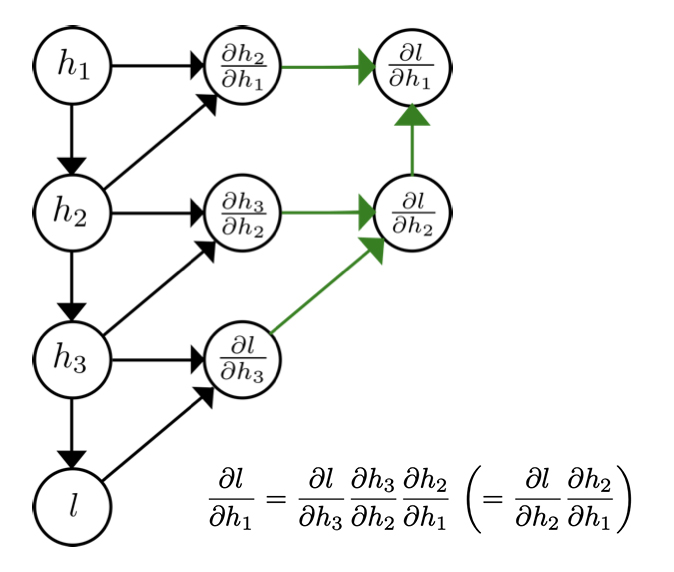
\includegraphics[width=0.7\columnwidth]{src/comp-graph.jpg}
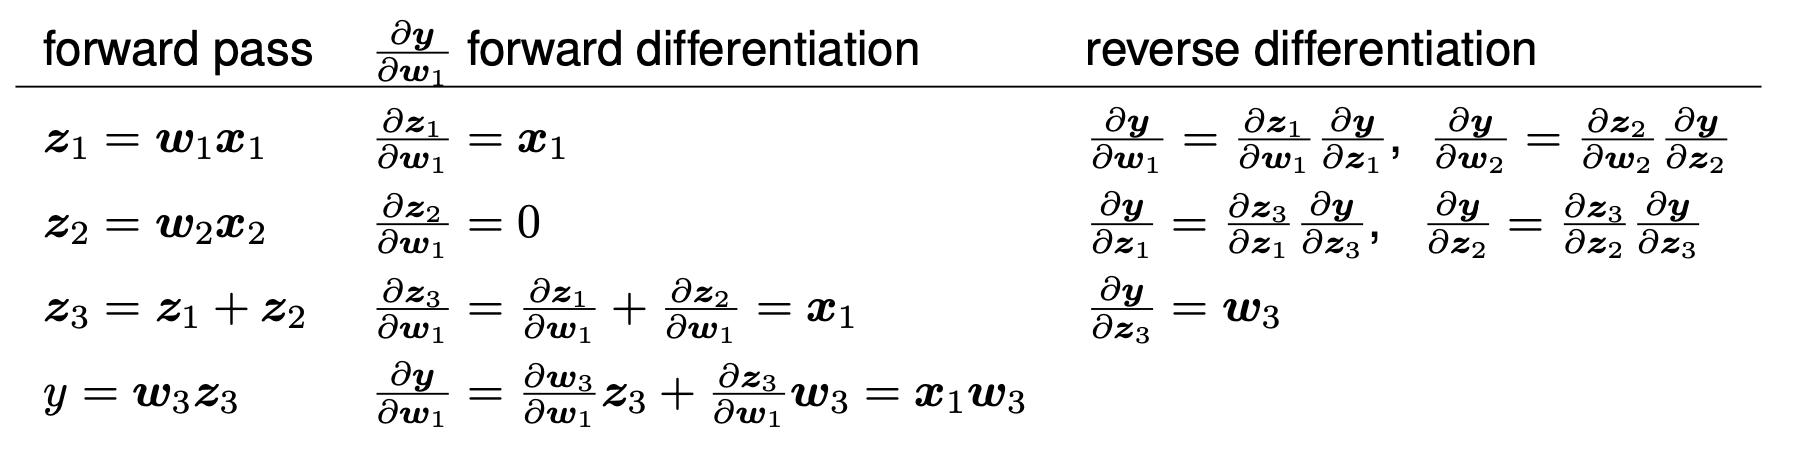
\includegraphics[width=\columnwidth]{src/diff-modes.png}

Forward prop: $O(\#params)$

Backward prop: $O(\#outputs)$
\section*{Chapter 7: Rectified Networks}
%\section*{Probabilities}
%\subsection*{Expect, Var, Cov, Bay}
%$\E[X]=\int_{\Omega}xf(x)\di x=\int_{\omega}x\Prob[X{=}x]\di x$ \\
\subsection*{Rectified Units}
\textbf{ReLU: } $(x, \theta) \mapsto (x\cdot\theta)_{+} = \max\{0, x\cdot\theta\}$. Convention: $\partial(z=0)_+ = 0$. Its benefit is that gradient does not vanish due to saturation: $\partial (z)_+ = 1 (\forall z > 0)$

Efficient backprop: $\partial(z_{lj}=0)_+ = 0 \implies \nabla_{\theta_{lj}}z_{lj} = 0$

\textbf{Absolute Value Unit: } $(x, \theta) \mapsto |x\cdot\theta|$

Relation: $(z)_+ = \frac{1}{2}(|z|+z)$ and $|z| = 2(z)_+-z = (z)_+ + (-z)_+$

\textbf{Smooth ReLU Approximations}

\textbf{Softplus} $\in (0; \infty)$:  $(x;\theta) \mapsto \ln(1+exp[x\cdot\theta])$

\textbf{elu} $\in (-1; \infty)$: 

$
(x, \theta) \mapsto =\begin{cases}
			x\cdot\theta & \text{if } x\cdot\theta \geq 0\\
            exp[x\cdot\theta] - 1 & \text{else}
		 \end{cases}
$

\textbf{Leaky ReLU} $\in \mathbb{R}$: 

$
(x, \theta) \mapsto =\begin{cases}
			x\cdot\theta & \text{if } x\cdot\theta \geq 0\\
            \epsilon x\cdot\theta & \text{else}
		 \end{cases}
$

\subsection*{Piecewise Linear Approximation}
\textbf{Thm:} Piecewise linear functions are dense in $C([0; 1])$

\textbf{Thm:} A piecewise linear function with m pieces can be written as: $g(x) = ax+b + \sum_{i=1}^{m-1}c_i(x-x_i)_+ = a'x+b'+\sum_{i=1}^{m-1}c_i'|x-x_i|$

\textbf{Corollary: } Networks with one hidden layer of ReLU or absolute value units are universal function approximators.

\textbf{Thm:} Every continuous piecewise linear function $g: \R^n \mapsto \R$ can be written as a signed sum of k-Hinges with $k\leq n+1$ -> Exact (not approx). Maxout units are $k$-hinge functions.

\textbf{Thm:} Maxout networks with two maxout units are universal function approximators.

\textbf{Polyhedral functions:} continuous piecewise linear functions that are also convex.

\textbf{Thm:} Every continuous piecewise linear funciton $f$ can be written as the difference of two polyhedral functions.

The minimal non-linearity needed to ensure universality are two maximum operations over finite sets.

\subsection*{Number of Linear Regions}

\section*{Chapter 8: Optimization}
%\section*{Probabilities}
%\subsection*{Expect, Var, Cov, Bay}
%$\E[X]=\int_{\Omega}xf(x)\di x=\int_{\omega}x\Prob[X{=}x]\di x$ \\
\subsection*{Objectives}
\textbf{Squared loss:} $l_{y}(\nu) = \frac{1}{2} \|y-\nu\|^2 $. Assumes isotropic Gaussian noise for outputs. Do not need output activation ($\nu = z$). $\partial l_y(\nu) = \nu - y$. 

\textbf{Zero-one loss:} $l_{y}(\nu) = 0 \text{ if } \nu=y \text{ else } 1$. The output unit can be seen as a max-unit on top of linear scores: $\nu = \argmax_j{z_j}$. Problem: lacks gradient info -> hard to optimize. Used to evalulate accuracy.

To avoid optimizing the zero-one loss, use surrogates. Usually, $z$ is turned into class probs using $\nu = \sigma^{max}(z)$.

\textbf{Binary cross-entropy: } $l_{y}(z)=-y\cdot \ln{\sigma(z)} - (1-y)\cdot \ln{1-\sigma(z)}$. $\equiv$ to max the log-likelihood.

\textbf{For m classes: } $l_{y}(z)=-\ln{\sigma_{y}^{max}(z)} = -z{y} + \ln({\sum_{j=1}^m \exp{[z_j]}})$. If soft targets: $l_{y}(z)=-\sum_{j=1}^m y_j\ln(\sigma_j^{max}(z)))$

\textbf{Hinge loss: } $l_y(z) = \max\{0, 1-yz\} = (1-yz)_+$

\subsection*{Probabilistic Loss Functions}
We can defined loss functions when models make probabilistic predictions. Assume prob. model over $\mathcal{Y}$ with parameter $\nu$.

\textbf{Log-likelihood loss: } $l_y(\nu) = -\log p(y;\nu)$

\textbf{Gaussian model: } $l_y(\nu) = \frac{1}{2}\|y-\nu\|^2 + const$

\textbf{Exponential model: } $l_y(\nu) = -y\cdot\nu + \psi(\nu) + const$

\textbf{Poisson model: } $l_y(\nu) = \nu - y\log\nu + const$

\subsection*{Gradient Descent}
True risk $R(\theta)=\mathbb{E}_p[l_y(F(x;\theta))]$ is estimated by empirical risk $R_s(\theta)=\frac{1}{s}\sum_{t=1}^s l_{y^{t}}(F(x^t;\theta))$

\textbf{Update iteration: } $\theta^{k+1} = \theta^k - \alpha\nabla f(\theta^k)$

\textbf{Gradient flow: } $\dot{x} = -\nabla f(x)$. We can think of the update interation as numerical integration of the gradient flow: ideal trajectory to be approximated by GD. As $\alpha$ gets smaller, we get closer to it.

\textbf{Convergence Theorem:} for a $\mu$-strongly convex, L-smooth function $f$, the gradient iterates $\theta^k$ with $\alpha\leq\frac{1}{L}$ converge to the unique minimizer $\theta^{*}$ at rate $\|\theta^k - \theta^{*}\|^2 \leq (1-\alpha\mu)^k\|\theta^0 - \theta^{*}\|^2$. For non-convex case we can prove conv. to an $\epsilon$-stationary point where $\|\nabla f(x)\| \leq \epsilon$

\textbf{Thm:} Let $f$ be convex, diff. and L-smooth. Then, with $\alpha\leq\frac{1}{L}$, the suboptimality along GD iterates decays like: $f(\theta^k) - f(\theta^*) \leq \frac{1}{2\nu k}\|x^0-x^*\|^2$ -> Cannot ensure conv to $\theta^*$ but bound optimality.

\subsection*{Stochastic Gradient Descent}
$\theta^{k+1} = \theta^k - \alpha_{k}\nabla f_{I(k)}(\theta^k), I(k) \sim Unif\{1,...,k\}$

To reduce variance, use minibatches: $\theta^{k+1} = \theta^k - \alpha_{k} \cdot \frac{1}{|S_k|}\sum_{j\in S_k}\nabla f_{j}(\theta^k)$

\subsection*{Constant learning rate}
The schedule $\alpha_k \propto 1/k$ is good in theory but slow convergence. Constant $\alpha$ can work. A small enough constant $\alpha$ can get arbitrary close to the optimum.

\subsection*{Momentum and Adaptivity}
\textbf{Nesterov's Accelerated Method: } $y^{k+1}=\theta^k + \beta(\theta^{k}-\theta^{k-1})$, $\theta^{k+1} = y^{k+1}-\alpha\nabla f(y^{k+1})$
\textbf{Heavy Ball (GD with mom): }$\theta^{k+1} = \theta^{k} - \alpha\nabla fx^k + \beta (x^k - x^{k-1})$, $\beta\in(0,1)$

\textbf{AdaGrad}. Adapt $\alpha$ per parameter or direction.

$\gamma^k = \eta\gamma^{k-1} + (1-\eta)[\nabla f(x^k) \odot \nabla f(x^k)]$

$x^{k+1} = x^k - \alpha\Lambda^k\nabla f(x^k)$ where

$\Lambda^k = diag(\lambda_i^k)$ with $\lambda_i^k = \frac{1}{\sqrt{\gamma_i^k} + \delta}, \delta>0$

Each $\gamma_i^k$ is the sum of the squares of the i-th parameters partial derivatives along the iterates $x^0, ..., x^k$

\textbf{Adam}. $\alpha$ is adapted per parameter as in AdaGrad but includes momentum term by exponentially decaying mean over the gradient history.

$\theta^{k+1} = \theta^k - \frac{\alpha}{1-\beta^k}m^k$ where $m^k = \beta m^{k-1} + (1-\beta)\nabla f(x^k)$ with $\beta\in[0,1]$ and $m^0=0$.
$(1-\beta^k)$ is a bias correction. $\alpha$ is computed as in AdaGrad.

\textbf{Compressed Stochastic Gradients.} Reduce computational and communication complexity. Simple approach \textbf{signSGD}:
$\theta^{k+1}=\theta^{k}-\alpha_ksign(\nabla f_{I(k)(x^k)})$ -> Biased estimate of gradient but still may work.
\section*{Chapter 9: Convolutional Networks}
%\section*{Probabilities}
%\subsection*{Expect, Var, Cov, Bay}
%$\E[X]=\int_{\Omega}xf(x)\di x=\int_{\omega}x\Prob[X{=}x]\di x$ \\
\subsection*{Convolutions}
\textbf{Convolution:} $(f*h)(u) = \int_{\mathbb{R}} h(u-t)f(t)dt = \int_{\mathbb{R}} f(u-t)h(t)dt = (h*f)(u)$ 

\textbf{Conv. is shift equivariant:} $f_{\Delta}*h = (f*h)_{\Delta}$

\textbf{Discrete conv.:} $(f*h)[u] = \sum_{t=-\infty}^{\infty}f[t]h[u-t]$

\textbf{Cross-correl.:} $(h\star f)(y) = \int_{\mathbb{R}} h(t)f(y+t)dt$

\textbf{2-D:} $(F*G)[i,j] = \sum_{k=-\infty}^{\infty}\sum_{l=-\infty}^{\infty}F[i-k, i-l] \cdot G[k,l]$

\subsection*{CNNs}
\textbf{Pros}: param sharing, more efficient, translation equivariance, sparse connectivity. \textbf{Cons}: not all data is trans. equiv. and receptive field makes it hard to connect distant features.

\textbf{Padding.} Used to handle borders. \emph{Same padding} pads with zeros and ensures output is of same size (breaks transition equivariance). \emph{Valid padding} only applies conv in the available signal (conv is exact but reduces size). \emph{Other ideas} e.g. reflecting borders to keep transition equivariance.

\textbf{Receptive fields}. CNNs units only have info about close points. By increasing depth, the receptive field increases and can reach further info.

\textbf{Pooling}. Used to locally combine activities by applying a function on each window e.g. max or avg.

\textbf{Strides}. Sub-sampling to reduce size of feature maps. Apply kernel (or pooling) each n pixels. Loss of info.

\textbf{Channels}. Learn multiple filters/kernels per layer. Add dimensions.

\subsection*{CNNS in CV}
Usually use RelU or Leaky ReLU as activation. Vanishing gradients with depth. They have a pyramidal architecture: stack convs reducing resolution while increasing channels.

\textbf{AlexNet}. Pyramidal CNN arch (1.3M+ params) + 3FC (177M+ params)

\textbf{VGG}. Very deep CNN. Only uses convs and it is transition invariant. Uses kernels 3x3 and takes the size down to $1\times N_{classes}$ and apply softmax.

\textbf{Inception}. Uses 1x1 conv to reduce input size by combining info across channels. Concatenates output from diff filter sizes to learn more. Includes sofmax layers at intermediate steps to ease backprop and avoid vanish grads.

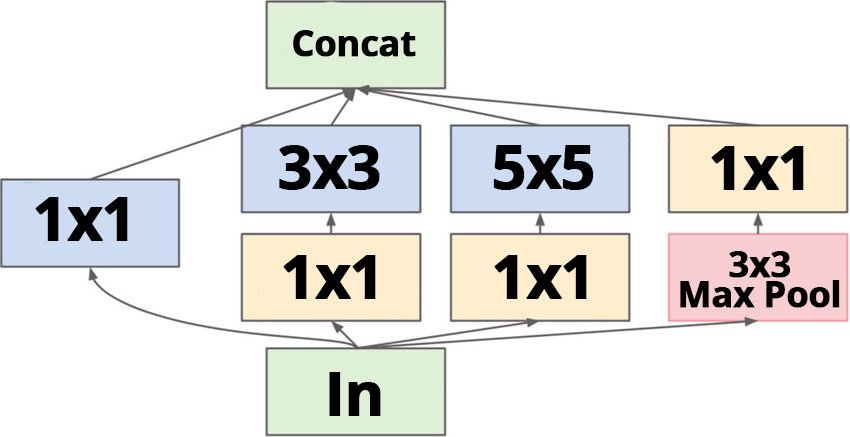
\includegraphics[width=0.6\columnwidth]{src/custom-inception.jpg}

\subsection*{CNNs shapes and parameters}
Given an input $(N, C_{in}, H_{in}, W_{in})$, the output of the conv. is $(N, C_{out}, H_{out}, W_{out})$:

$H_{out} = \lfloor \frac{H_{in}+2 \cdot padding[0] - (kernel\_size[0] - 1)}{stride[0]} + 1 \rfloor $

$W_{out} = \lfloor \frac{W_{in}+2 \cdot padding[1] - (kernel\_size[1] - 1)}{stride[1]} + 1 \rfloor $

The \#params in a layer is: $weights+bias$:

$weights = C_{in} \cdot C_{out} \cdot kernel[0] \cdot kernel[1]$

$bias = C_{out}$

\subsection*{CNNs in NLP}
Map a set of symbols (chars, words, etc.) to a vector space (embedding). Then, apply CNN to the embedding space.

\textbf{Word2Vec}. Uses a log-bilinear model to predict prob. of word $\nu$ appearing in neighborhood of $w$. $p(\nu|w) = \frac{exp[x_w\cdot y_\nu]}{\sum_\mu exp[x_w\cdot y_\mu]}$. Requires summing over vocabulary $\mu$ (expensive). Can use negative sampling to avoid the sum. In this case we only predict prob of appearing together $p(1|\nu, w)$
\section*{Chapter 10: Recurrent Neural Networks (RNNs)}
%\section*{Probabilities}
%\subsection*{Expect, Var, Cov, Bay}
%$\E[X]=\int_{\Omega}xf(x)\di x=\int_{\omega}x\Prob[X{=}x]\di x$ \\
Given an observation sequence $x^0, ..., x^s$, we want to identify hidden activities $h^t = F(h^{t-1}, x^t, \theta)$. $F$ can be a RNN $F(h, x; \theta) = \sigma(Wh + Ux + b)$. We can produce outputs $y = H(h; \theta) := \sigma(Vh + c)$.

Gradients vanish (or explode) for long sequences.

\textbf{Bi-directional RNN}. Take into account future by a reverse order sequence $g^t = G(x^t, g^{t+1}; \theta)$.

\textbf{Deep RNN}. Stack different hidden states and connect output to last hidden layer. $h^{t,1} = F^1(h^{t-1, 1}, x^t; \theta^1), ... h^{t,l} = F^l(h^{t-1, l}, h^{t, l-1}; \theta^l)$.

\subsection*{LSTM}
Their goal is to overcome the main limitation of RNNs: they forget quickly. Define gated units that can learn long-term dependencies.
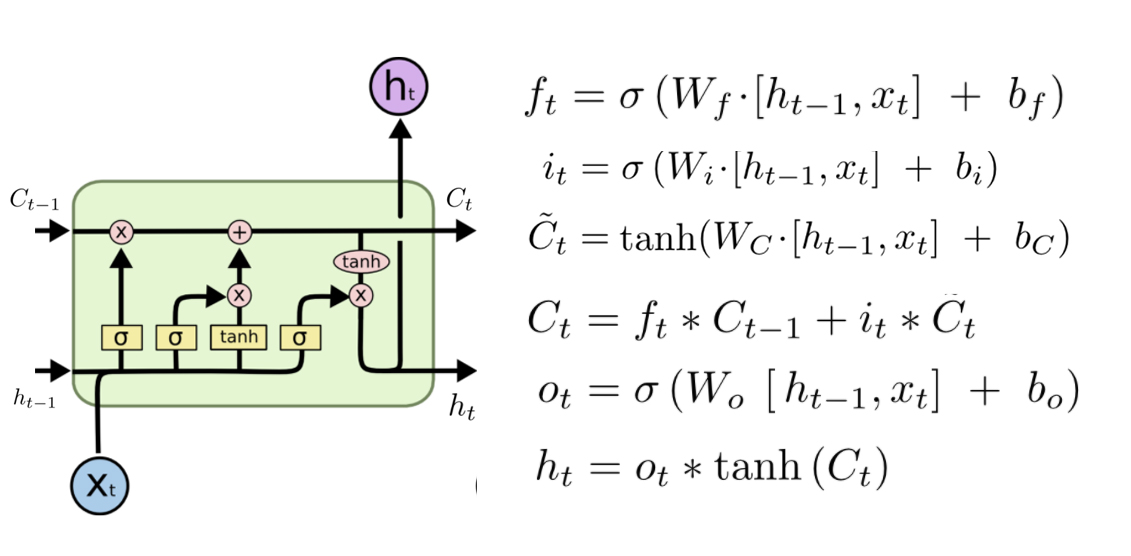
\includegraphics[width=\columnwidth]{src/lstm.jpg}
\subsection*{Gated memory units}
Simplified LSTM. Still difficult to train.
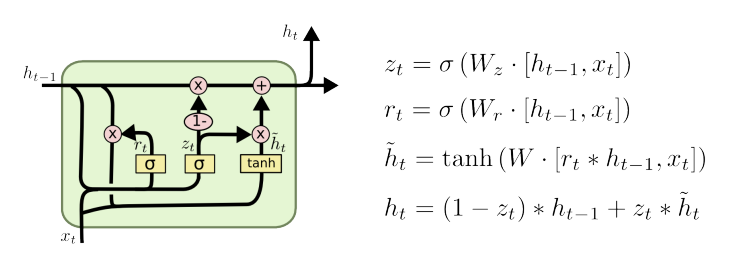
\includegraphics[width=\columnwidth]{src/gated-memory-units.png}

\subsection*{Learning sequences}
Goal: define cond. probability dist. over output sequence $y^{1:T}$ given inputs $x^{1:T}$ (special case: no input): $p(y^{1:T} | x^{1:T}) \approx \prod_{t=1}^Tp(y^t | x^{1:t}, y^{1:t-1})$.

A naïve RNN implementation would be: $x^{1:t} \xMapsto[]{F} h^t$; $h^t \xMapsto[]{H}\mu^t$; $\mu^t\xMapsto[]{H}p(y^t)$. The problem is that we assume $y^t$ is independent from $y^{t-1}$ (dependence through $h^t$). To overcome this, we can feedback previous outputs. 

\subsection*{Sequence-to-sequence learning}
Translate input sequence $x^{1:T}$ to $y^{1:T'}$. They might have diff. lengths and be unaligned. We build an encoder (RNN) that maps $x^{1:T} \mapsto z$ where $z=h^t$ (last hidden state). Then, a decoder maps $z \mapsto y^{1:T'}$. $z$ is "thought vector" that encodes the meaning of the sentence. It can be created from any model; e.g. a CV task.
\section*{Chapter 11: Deep Gradients}
\subsection*{Short connectivity}
Include skip connections to avoid vanishing gradients in deep networks. Instead of having $x'=\sigma(W_2\sigma(W_1x))$, we define $x'=\sigma(W_2\sigma(W_1x) + W'x)$. $W'$ is only used if there is a change in the shapes. Otherwise, $W'=I$

\subsection*{Dense connectivity}
Create dense blocks by concatenating channels from all previous layers. Use transition layers to reduce dimensionality after dense block.

\subsection*{Normalization}
Idea: normalize output of layers before activation.

\textbf{Batch norm.} Very effective and used in CV. Depends on batch size (larger is better) and not suitable for all arch. For each batch $I \subseteq [1,..., s]$ in a fixed layer $l$, compute:

Mean activity: $\mu^l:=\frac{1}{|I|}\sum_{t\in I}z^l[t]$

Vector of std: $\sigma_i^l := \sqrt{\delta + \frac{1}{|I|}\sum_{t\in I}(z^l[t]-\mu_i^l)^2}$

Norm activities: $\tilde{z}_i^l := \alpha_i^l \frac{z_i^l - \mu_i^l}{\sigma_i^l} + \beta_i^l$ where $\alpha, \beta$ are learned to regain representational power and achieve faster convergence.

\textbf{Layer norm.} Useful for RNN. Not consistent benefits across tasks. Works with any batch size, even 1. Follows same idea as BN.

$\mu^l[t] := \frac{1}{m^l}\sum_{i=1}^{m^l}z_i^l[t]$

$\sigma^l[t] := \sqrt{\delta + \frac{1}{m^l}\sum_{i=1}^{m^l}(z_i^l[t]-\mu^l[t])^2}$

$h[t] = f_1(\frac{g}{\sigma^l[t]} \cdot (a[t] - \mu[t]) + b)$
\section*{Chapter 12: Regularization and Augmentation}
%\section*{Probabilities}
%\subsection*{Expect, Var, Cov, Bay}
%$\E[X]=\int_{\Omega}xf(x)\di x=\int_{\omega}x\Prob[X{=}x]\di x$ \\
Regularization: aspect used to lower generalization error but not training error.

\textbf{Norm-based regularization}. Encode prior knowledge in the optimization; e.g. weights should be small: $R_\Omega(\theta; S) = R(\theta; S) + \Omega(\theta)$. First term is risk and second regularizer on $\theta$. Example 
$\Omega(\theta) = \frac{1}{2}\sum_{l=1}^{L}\mu^l\|\theta^l\|_p^2$

\textbf{Weigth Decay}. L2-reg on weights. 

$\nabla\Omega = \mu\theta$ or $\frac{\partial\Omega}{\partial\theta_{ij}^l} = \mu\theta_{ij}^l$

GD becomes: $\theta^{k+1} = ((1-\mu\eta)\theta^k - \eta \nabla R(\theta^k))$

\textbf{Early stopping}. Keep best set of weights during training based on val error.

\textbf{Ensemble Methods: bagging}. Comibne models trained on bootstrap samples. In practice, many duplicates and we sample $2/3$ of the data. At inference time, (weighted) average of all model outputs. Always beneficial but expensive.

\textbf{Knowledge distillation}. Given an accurate and complex model, train a target model which is cheaper but replicates it. To do that train the target model on training data + data labelled by the complex model. Allows to use even more data.

\textbf{Dropout}. Drop units in network with prob $p$. We avoid unique paths to get solutions. We can interpret dropout as building ensemble of different NN. We can use \emph{Weight rescaling} and scale weights by prob of being active: $\Tilde{\theta}_{ij} \leftarrow \pi_j^{l-1}\theta_{ij}^l$

\textbf{Data augmentation}. Enrich data with prior knowledge. We define transformations $\tau$ and apply them to each training sample: $(x, y) \mapsto (\tau(x), y)$. Also, can inject noise during training in inputs, weights or targets.

\textbf{Task augmentation}. Pre-train parts of the model on generic task. In \emph{self-supervised} learning, build aux tasks that allow to train models on unlabelled data. In \emph{Semi-supervised}, define a generative model w/ log-likelihood and optimize additive combination of supervised and unsupervised risk while sharing parameters.
\section*{Chapter 13: Theory of DNNs}

\textbf{Setting}:
$P$ over $\mathcal X\times\mathcal Y$,
hypothesis class $\mathcal F$,
true risk: $\mathcal R(f):=\mathbb E[\mathds{1}_{\{f(\mathbf x)\neq y\}}]$,
empirical risk: $\mathcal R_n(f)=\frac 1 n \sum_{i=1}^n \mathds{1}_{f(\mathbf x_i\neq y_i)}$,
true risk minimizer $f^*$,
empirical risk minimizer $f_n$,
$\mathcal R(f^*)\leq \mathcal R(f_n)$,
$\mathcal R_n(f_n)\leq \mathcal R_n(f^*)$

We represent bounds as: $\mathbb P(R(f) \leq R_n(f) + \text{Complexity term}) \geq (1-\delta) \to$ Probabilistic because $R_n(\cdot)$ depends on random draws.

\textbf{Hoeffding's inequality}: $Z_i\in [a, b]$ i.i.d.

$\mathbb P
\left[
    \left|
        \frac 1 n \sum_{i=1}^n
            Z_i - \mathbb E[Z]
    \right|
    > \epsilon
\right]
< 2 \exp
    \left(
        -\frac
            {2n\epsilon^2}
            {(b-a)^2}
    \right)
$

Intuition: prob of having large deviations between true and empirical mean is bounded. The more data, the closer we might expect to be. 

\textbf{Union bound}:
$
\mathbb P[C_1\bigcup ... \bigcup C_N] \leq
\sum_{i=1}^N \mathbb P [C_i]
$

The prob of union of events is larger than sum of their probs.

\textbf{Scattering coefficient}:
$
\mathcal S_{\mathcal F} := \sup_{(\mathbf x_1, ..., \mathbf x_n)}
\left|
    \{
        (f(\mathbf x_1), ..., f(\mathbf x_n)) : f\in\mathcal F
    \}
\right|
$

Intuition: how many diff functions of the data can my function class represent?

\textbf{Shatter}: if $\mathcal S_{\mathcal F}(n) = 2^n$ then $\mathcal F$ shatters set.

If for a fixed n, we can classify data points in all the possible ways ($2^n$), then $\mathcal F$ shatters the set.

\textbf{VC dimension}: largest $n$ for which $\mathcal S_{\mathcal F}(n) = 2^n$;
VC dim of linear classifier in 2d: 3;
VC dimension of binary linear classifier with $d$ weights: $d+1$

If VC dim is $n^*$, $S_{\mathcal F}(n)$ grows sub-exponentially with $n$ when $n>n^*\to$ VC dim grows sub-linearly.

Conclusion: finiteness of the VC dim ensures that emp. risk converges uniformly over $\mathccal$

\textbf{Symmetrization lemma}:

\textbf{Sauer's lemma}: for a function class $\mathcal F$ with VC-dim($\mathcal F$) $\leq d$ and $n>d$, then: $\mathcal S_{\mathcal F}(n) \leq (\frac{en}{d})^d$

\textbf{Thm}: the VC-dim of a binary linear classifier (perceptron) with d weights and 1 bias term is: $d+1$.

\textbf{Puzzling capacity of NN}

NN are powerful function approximators.

- When incresing hidden units, train error goes to 0 but there's no overfitting because test error also keeps decreasing.

- No matter what we use as data, training goes to 0 as hidden units increase. They can even fit random labels (no generalization).
\section*{Chapter 14: Attention}
%\section*{Probabilities}
%\subsection*{Expect, Var, Cov, Bay}
%$\E[X]=\int_{\Omega}xf(x)\di x=\int_{\omega}x\Prob[X{=}x]\di x$ \\
\subsection*{Gating function}
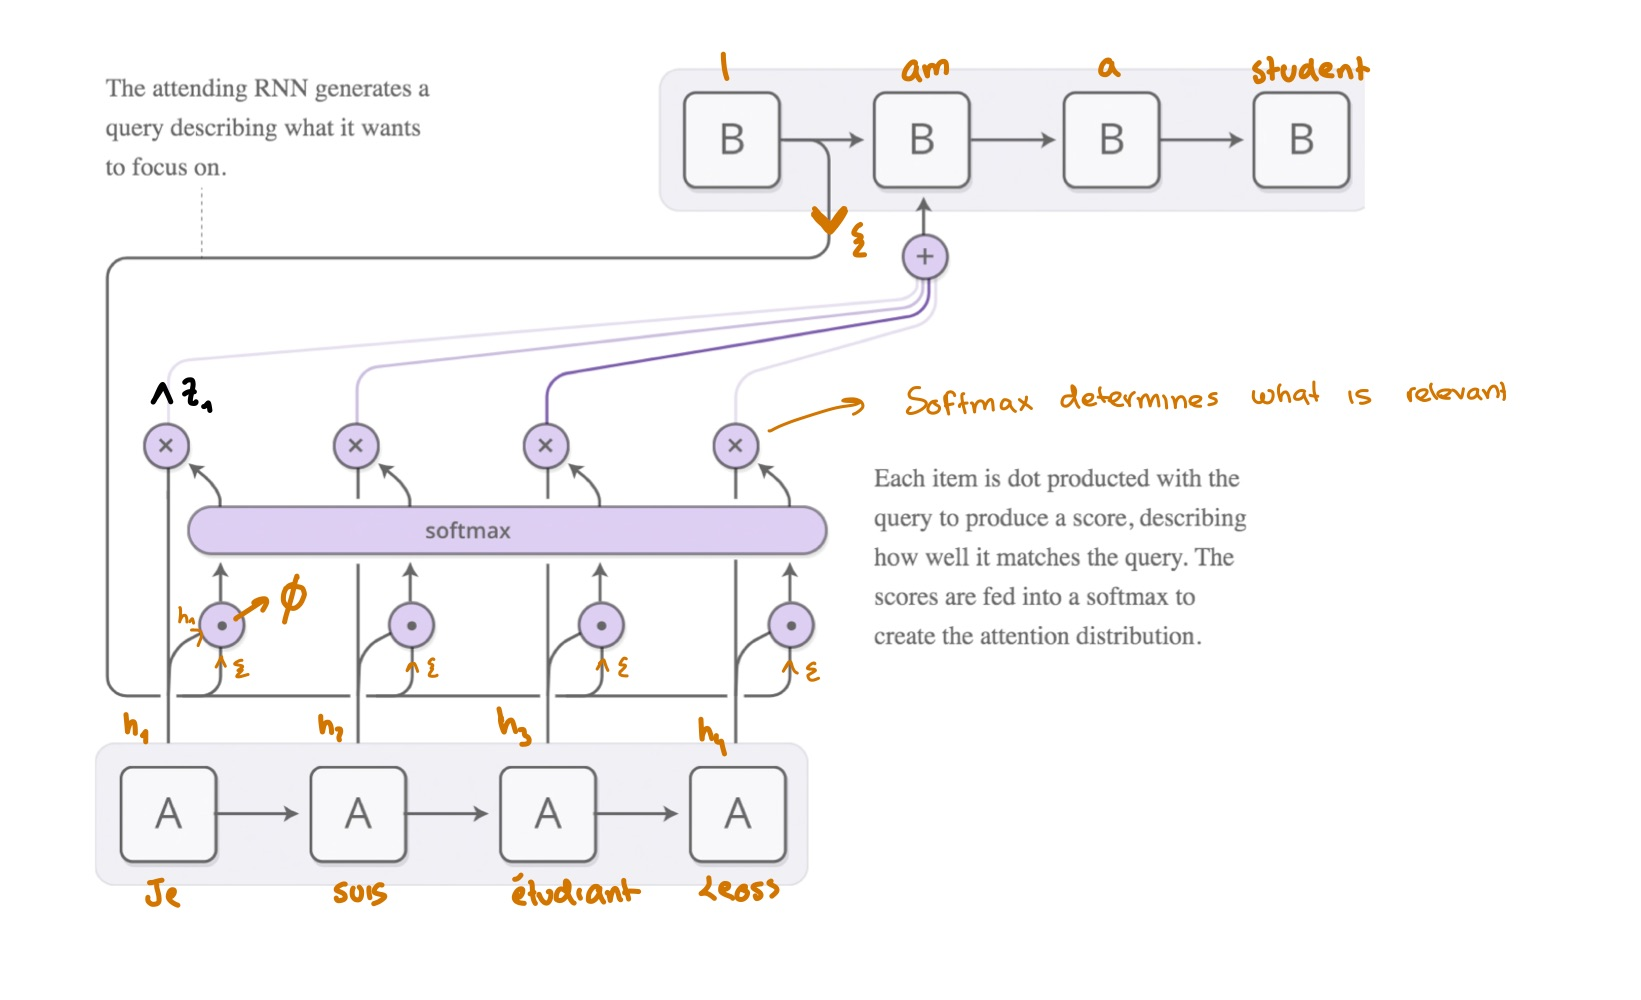
\includegraphics[width=\columnwidth]{src/gating-function.jpg}
Used in combination with RNNs to focus on relevant parts of the input depending on the desired output. Given all hidden states from the encoder ($h_e^1, ..., h_e^s$), the decoder defines a query vector $\xi \in \R^n$. Then, a function is applied between each hidden state and the query vector (can be their dot product) and a softmax on these outputs creates the attention distribution. Finally, probabilities are multiplied by their corresponding $h_e$ producing "read-outs" ($z_1, ..., z_t$) that are used as input to the decoder $(h_d^r, z^r) \mapsto y_d^{r+1}$.

\subsection*{Transformers}
Attention is all you need. Remove RNNs for efficiency. They use a stack of encoders and decoders. Each encoder is (self-attention layer + feed forward NN). Each decoder is (self-attention layer + encoder-decoder attention + feed forward NN).

\subsection*{ELMO: Contextualized Word Embeddings}
Construct embeddings that reflect context. A CNN takes as input the embedding of each input character and creates a representation for each word. Then, a bi-directional LSTM modify the representation of each word based on the context and at the end, a linear combination of all hidden layers yields the ELMO representation. Unsupervised training: predict next word.
\section*{Chapter 15: Learning on Graphs}
A graph is made of a set of nodes $\mathcal V = \{v_1, \hdots, v_n\}$ and a set of edges $\mathcal E$ that encode dependencies.

Given a connected, undir., weighted graph $G=\{\mathcal{V, E, W}\}$ and $\x$, vector containing vertex values:
- Adjacency matrix (A) contains weight of edges between nodes.

- Degree matrix (D): diag matrix with incoming weights for each node: $D_{ii} = \sum_{j}A_{i,j}$.

- \textbf{Edge derivative: } $\nabla_{i,j}\x = \frac{\partial\x}{\partial e_{i,j}} = A_{i,j}(x_j-x_i)$

- Laplacian: $L_x = \nabla^\top\nabla\x = D-A$

- Norm Lap.: $L' = \mathbb{I}-D^{-1/2}AD^{-1/2} = D^{-1/2}LD^{-1/2}$. Its max eigenvalue is 2.

- $L = \nabla^\top\nabla$ is symmetric positive semi-definite $\to L=U\Lambda U^\top$ where $U$ is the graph Fourier basis w/ transform $\hat{\x} = U^\top\x$ and inverse transform $\x = U\hat{\x}$

Convolution in graphs can be defined in 3 ways:

\subsection*{1. Spectral convolution}
It generalizes traditional convolution. Multiplication in spectral domain. For a kernel $h$, the conv. of $h$ and $\x$ is $h(L)\x := Uh(\Lambda)U^\top\x $

Needs full Laplacian decomposition $\to O(|\mathcal V|^3)$.

Can use polynomial kernels $p(t) = \sum_{i=0}^K\alpha_it^i$. Then filtering becomes: $p(L)x := Up(\Lambda)U^\top\x = U(\sum_{i=0}^K\alpha_i\Lambda^i)U^\top\x = \sum_{i=0}^K\alpha_iL^i\x$. Assuming L is sparse, complexity scales with \#edges: $O(|\mathcal E|)$

The order of the polynomial defines the size of the neighborhood to gather info. In practice, given $c_{in}$ channels and desired $c_{out}$ channels, we learn $c_{in} \cdot c_{out}$ polynomial kernels shared for all nodes, add bias $\beta_j$. Sum over channels to keep hidden variables under control. \#params $= c_{in}\cdot c_{out}\cdot(K+1)\cdot c_{out}$

\subsection*{2. Vertex convolution}
Define conv generically using a shared operation for all edges and nodes and an aggregation (AGG) and combination (COM) function. A convolution layer is defined:

- $Z_i^{(k)} = \text{AGG}(\{e(X_i^{k}, X_j^{(k)}, A_{i,j}): v_i \sim v_j\})$

- $X_i^{(k+1)} = \text{COM}(Z_i^{k}, h(X_i^{(k)}))$

where $e$ is a shared function for all nodes (MLP) and $h$ is also shared. Everything is done in vertex domain.

\subsection*{3. Graph Convolutional Networks}
$1^{st}$ order spectral conv (mix of prev approaches). 

Apply MLP on the nodes with shared parameters and coupling activities of neighboring units: $\X^{l+1} = \sigma(W^l\X^l\mathbf Q)$ where $\mathbf Q$ is the coupling matrix. Usual choice: degree-normalized matrix $Q=\tilde D^{-\frac 1 2}\tilde A\tilde D^{-\frac 1 2}$; augmented adjacency matrix $\tilde A := A + \mathbb{I}_n$, diagonal degree matrix $\tilde D$ of $\tilde A$.
\section*{Chapter 16: Factor Analysis}
Find latent variables $(\z_1, \hdots, \z_m)$ s.t they represent observations $(\x_1, \hdots, \x_n)$ for $n>m$. They are releated through a matrix of coefficients (need to learn).

Given latent variable $\z \sim p(\z)$, observe $\x$ with likelihood $p(\x|\z)$: (1) set a prior on $\z: \z\sim N(0, I)$ and (2) model $\x$ according to a linear model: $x = \mu + W\z + \eta$ where $W$ captures relation between $\x$ and $\z$ and $\eta \sim N(0, \Sigma), \Sigma:=\text{diag}(\sigma_1^2, \hdots, \sigma_n^2)$ is random noise.

$\mu$ can be computed using MLE: $\hat\mu = \frac{1}{t}\sum_{i=1}^t\x_i$

Then, $\x \sim N(\mu, WW^\top + \Sigma)$

\subsection*{Moment Generating Functions (MGF)}
The MGF of random vector $\x$ is 

$M_\x : \R^n \to \R, M_\x(t):= \E_\x\exp{[t\cdot\x]}$.

It represents moments $(k_1, \hdots, k_n)$ of $\x$ as $\E[x_1^{k_1} \hdots x_n^{k_n}] = \frac{\partial k}{\partial t_1^{k_1} \hdots \partial t_n^{k_n}}M_\x |_{t=0}$ 

Idea: once we have MGF, computing any moment is easy. Given RV $\x$ and $\y$ with $M_\x$ and $M_\y \to$ $M_{\x+\y} = M_\x \cdot M_\y$.
\section*{Chapter 17: Adversarial Attacks}

\textbf{Adversarial robustness} can be evaluated in two ways: (1) given $\epsilon \geq 0$, return proportion of input samples for which there exists no adv perturbation with $\|r\|_p \leq \epsilon$. (2) return avg norm of minimal adversarial perturbations for each sample.

\textbf{Adversarial attack def: } Let $k : \R^d \to \{1, \hdots, C\}$ be a C-class classifier and $\x \in \R^d$ be an input. We define adv perturbation for $\x$ as finding $r\in\R^d$ s.t.:

- $k(\x+r) \neq k(\x)$

- $\x + r$ is similar to $\x$

- $\|r\|_p$ is small

\textbf{Minimal adv perturbation}: $\argmin_r \|r\|_p$ s.t. $k(\x+r) \neq k(\x)$ $\to$ break into problems that can be analitically solved.

For a binary linear classifier $f(x) = W^\top\x + b$ and $k(x) = 1$, solve: $\argmin_r \|r\|_p$ s.t. $(f_1(x+r) - f_2(x+r)) < 0 \equiv (w_1-w_2)^\top + f_1(\x) - f_2(\x) < 0$

\textbf{Hölder's ineq}: $r = \frac{f_1(x) - f_2(x)}{\|w_2-w_1\|_q^q}[(w_1-w_2) \odot \text{sign}(w_1-w_2))]^{\odot(q-1)}\odot\text{sign}(w_2-w_1)$. In 2-D, simplifies to: $r = \frac{f_1(x) - f_2(x)}{\|w_2-w_1\|_2^2}(w_2-w_1) \to$ projection to decision boundary.

For many classes, solve $r_i$ for $i\neq 1$ and choose $r = \argmin_{\{r_i\}} \|r_i\|_2$

\subsection*{DeepFool}
Since there is closed solution for linear classifier, solve initial problem by a sequence of linearized problems. In the binary case: $\argmin_r \|r\|_p$ s.t. $(\nabla_xf_1(x) - \nabla_xf_2(x))^\top r + f_1(x) -f_2(x) < 0 \to$ first order taylor exp. Solve iter until find sol.

\subsection*{Adversarial training}

\textbf{Robust opt}: $\min_\theta \max_{\|\mathbf r\|_p\leq \epsilon} \ell(y, f_\theta(x+r))$ 

\textbf{Danskin's Thm}: Intuition: we can first find max perturbation and then minimize loss wrt it. Let $r^*(\boldsymbol \theta):=\argmax_{\|\boldsymbol r\|\leq \epsilon} l(\boldsymbol \theta, \mathbf r)$, then $$\nabla_{\boldsymbol\theta}\max_{\|\mathbf r\|\leq \epsilon} g(\boldsymbol\theta, \mathbf r)=\nabla_{\boldsymbol\theta}l(\boldsymbol\theta, \mathbf r^*(\tilde{\boldsymbol\theta}))|_{\boldsymbol{\tilde\theta}=\boldsymbol\theta}$$ 

Maximization is usually solved using \textbf{PGD}. 

- $p=2 \to \tilde r^{s+1} \leftarrow r^s + \alpha \nabla_x l(f_\theta(x+r^s), y)$. Then, $r^{s+1} = \Pi_\epsilon^2(\tilde r^{s+1}) \to$ projection

- $p=\infty \to \tilde r^{s+1} \leftarrow r^s + \alpha \text{sign}(\nabla_x l(f_\theta(x+r^s), y))$. Then, $r^{s+1} = \Pi_\epsilon^\infty(\tilde r^{s+1})$

\textbf{FGSM} $\equiv$ 1-iter $l_\infty$-PGD. Weak.
\section*{Chapter 18: Variational Autoencoders}
%\section*{Probabilities}
%\subsection*{Expect, Var, Cov, Bay}
%$\E[X]=\int_{\Omega}xf(x)\di x=\int_{\omega}x\Prob[X{=}x]\di x$ \\
\textbf{Definetti's Thm}: for exchangeable data, we can decompose it by a latent variable model $p(x_1, \hdots, x_N) = \int\prod_{i=1}^{N}p_\theta(x_i|z)p_\theta(z)dz$. Problem: assumption of ind.

Clasically, define complex models via marginalization of a latent variable model: $p_\theta(x) = \int p_\theta(x,z)dz$. This posterior is computed using sampling methods or variational inference (ELBO).

\subsection*{Variational autoencoders}
Generalize factor analysis with depth. Given a "noise" variable $z \sim N(0, \mathbb I)$, propagate through DNN s.t. $\x = F(z) = (F^L \circ \hdots \circ F^1)(z)$. Encoder $\x \xMapsto[]{q_\phi} (\mu, \Sigma)$ and decoder $\z \xMapsto[]{p_\theta} \tilde{x}$ where $\z\sim (\mu, \Sigma)$.

To learn F(z), cannot use MLE because DNN does not provide density. We use a DNN that approximates the posterior $p_\theta(\z | \x) \approx q_\phi(\z | \x)$. The marginal log-likelihood (to be max) is $p_\theta(\x^{(1)}, \hdots, \x^{(N)}) = \sum_{i=1}^N \log p_\theta(\x^{(i)})$ where $\log p_\theta(\x^{(i)}) = KL(q_\phi(\z|\x^{(i)}) \| p_\theta(\z|\x^{(i)})) + \mathcal L(\theta, \phi; \x^{(i)})$. The first term is intractable but 
$KL \geq 0 \to$, max the expression is equiv to max the second term (ELBO):

$\log p_\theta(\x^{(i)}) \geq \mathcal L(\theta, \phi; \x^{(i)}) = \E_{q_\phi(\z|\x)}[\log p_\theta(\x, \z) - \log q_\phi(\z|\x)] = \E_{q_\phi(\z|\x^{(i)})}[\log p_\theta(\x^{(i)} | \z)] - KL(q_\phi(\mathbf z | \x^{(i)}) \| p_\theta(\mathbf z))$

\textbf{General Stoch Grad Variational Bayes}

$\mathcal{\tilde{L}}^A(\theta, \phi; \x^{(i)}) = \frac{1}{L}\sum_{l=1}^L\log p_\theta(\x^{(i)}, \z^{(i, l)}) - \log q_\phi(\z^{(i,l)}|\x^{(i)})$ with $\z^{(i,l)} = g_\phi(\epsilon^{(i,l)}, \x^{(i)})$ and $\epsilon^{(l)} \sim p(\epsilon)$
\section*{Chapter 19: Generative Models}
Given data coming from unknown distribution $p(x)$, learn $p_\theta(x)$ so that they are indistinguishable. Main challenges: mode collapse $p(x) >> p_\theta(x) \gtrapprox 0$ (all images look the same) and incorrect data $p_\theta(x) >> p(x) \gtrapprox 0$.

\subsection*{Generative Adversarial Networks}
Transform density estimation into classification. Idea: discriminator (D) cannot distinguish between true and generated samples by G:

$\tilde p_\theta(\x, y) = \frac{1}{2}(yp(\x) + (1-y)p_\theta(\x))$

\textbf{Bayes optimal classifier:} $q_\theta(x) = \frac{p(\x)}{p(\x) + p_\theta(\x)}$

Train generator by min logistic likelihood: $\theta \xMapsto[]{\min} l^*(\theta) := \E_{\tilde p_\theta} [y\ln q_\theta(\x) + (1-y)\ln(1-q_\theta(\x))]$

The objective that gets minimized is:

$\min_G\max_D L(D, G) = \E_{\mathbf x \sim p(\mathbf x)}[\log D(x)] + \E_{\mathbf z \sim p_\theta(\mathbf z)}[\log (1-D(z))]$ aka

$\E_{\frac{1}{2}(p+p_\theta)}[y\ln q_\theta(\x) + (1-y)\ln (1-q_\theta(\x))] = \E_{\frac{1}{2}(p+p_\theta)}[y\ln p(\x) + (1-y)\ln p_\theta(\x) - \ln(p(\x) + p_\theta(\x))] = -\frac{1}{2}H(p) -\frac{1}{2}H(p_\theta) + H(\frac{1}{2}(p+p_\theta))-\ln 2 = \text{JS}(p, p_\theta) - \ln 2 \to$ Jensen-Shannon div

Optimal class. is inaccesible, use NN $q_\phi : \x \to [0; 1]$

Define new objective via bound

$l^*(\theta) \geq \sup_{\phi\in\Phi} l(\theta, \phi)$

$l(\theta, \phi) := \E_{\tilde p_\theta}[y\ln q_\phi(\x) + (1-y)\ln(1-q_\phi(\x))]$

$\to \theta^* := \argmin_{\theta\in\Theta}\{\sup_{\phi\in\Phi}l(\theta, \phi)\}$

Use SGD (may diverge): $\theta^{t+1} = \theta^t - \alpha\nabla_\theta l(\theta^t, \phi^t)$

$\phi^{t+1} = \phi^t - \alpha\nabla_\phi l(\theta^{t+1}, \phi^t)$

Common trade-off: noisy samples but adequate representation of variability or faithful samples but lack of representation (mode dropping).

\subsection*{Normalizing flows}
Not as powerful as other generative models but they provide the likelihood. Goal: go from simple dist to complex and viceversa.

\textbf{Change of variable formula}. For a given RV $Z$ and $\x=g_\theta(z) \to p_X(\x) = p_Z(z) |\det(\frac{\partial g_\theta(z)}{\partial z^\top})|^{-1}$

or where $f_\theta(\cdot) = g_\theta(\cdot)^{-1}$: 

$p_X(\x) = p_Z(f(x))|\det(\frac{\partial f_\theta(x)}{\partial x^\top})|$

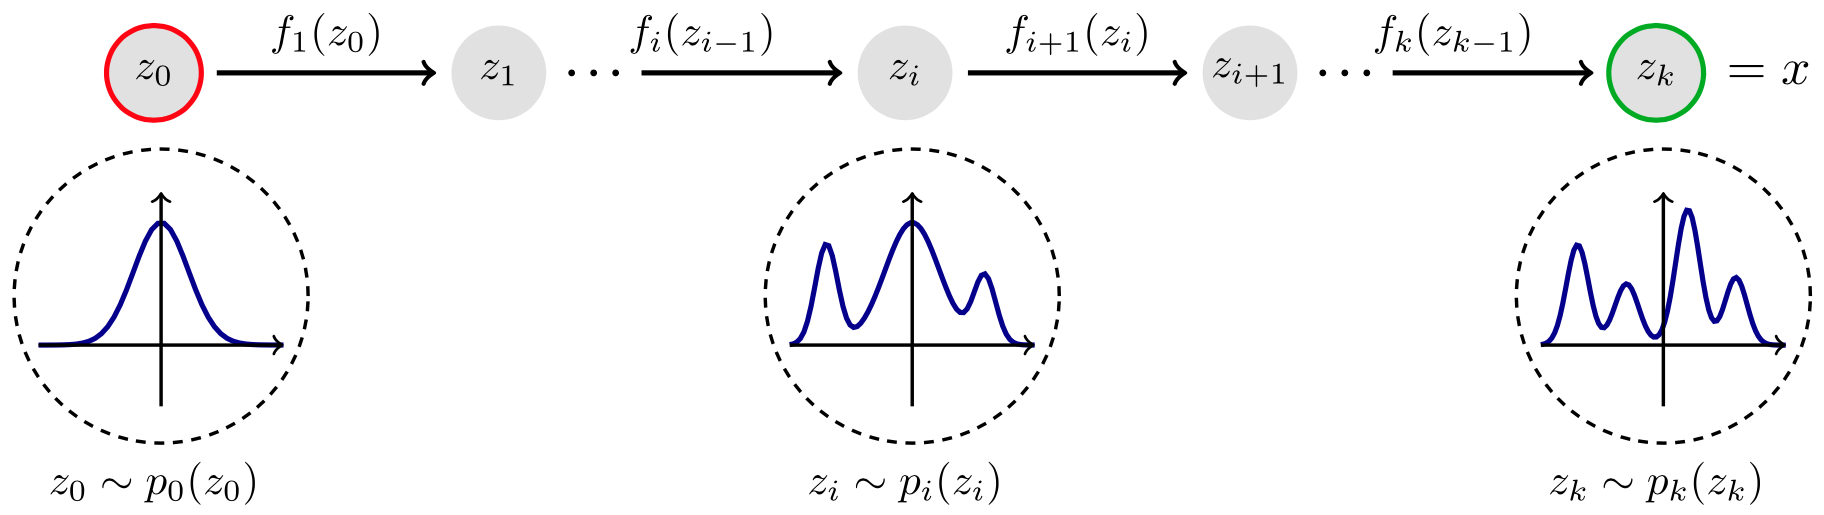
\includegraphics[width=\columnwidth]{src/normflows.png}

Normalizing flow is a bijection $F$ which is convenient to compute, invert and calculate $|\det(\partial F)|$. We use a stack of layers such that: 

- $F = F_L \circ \hdots \circ F_1$, $F^{-1} = F_1^{-1} \circ \hdots \circ F_L^{-1}$

- $\det(\partial F) = \prod_{l=1}^L \det(\partial F_l \circ \partial F_{l-1: 1})$

- $\det(\partial F^{-1}) = \det(\partial F)^{-1}$

- $\log p(\x|\z) = -\sum_{l=1}^L \log|\det(\partial F_l \circ F_{1:l-1})|$

\textbf{Linear flow}

Linear transform w/ invertible $A$: $F(z) = Az + b$, $\partial F = A$. It is equal to linear factor analysis if $z \sim N(0, \mathbb{I})$. Requires $O(n^3)$ to compute det and inv.

\textbf{(Tri-)Diagonal flows}. They use a diagonal matrix as $A$. In Triagonal, $A$ is upper or lower triagonal. Complexity decays but not very powerful.


% TODO commented this out because there were errors
%\subsection*{Probabilities}

$\E_{Y|X}[Y]=\E_{Y}[Y|X]$

$\E_{X,Y}[f(X,Y)]=\E_{X}\E_{Y|X}[f(X,Y)|X]$

$\E_{Y|X}[f(X,Y)|X]{=}\int_\mathbb{R}f(X,y)\Prob(y|X)\di y$

$\C(\X,\Y)=\E[(\X-\E[\X])(\Y-\E[\Y])] = \E[\X\Y^T]-\E[\X]\E[\Y]^T$

$\C(\mathbf{a}\X,\mathbf{b}\Y)=\mathbf{a}\C(\X,\Y)\mathbf{b}^T$

$P(A|B) = \frac{P(B|A) \cdot P(A)}{P(B)}$; $p(Z|X,\theta) = \frac{p(X,Z|\theta)}{p(X|\theta)}$

Vec. Var: $\mathbb V[\mathbf x]=\mathbb E[\mathbf x\mathbf x^T]-\mathbb E[\mathbf x]\mathbb E[\mathbf x]^T=\mathbb E[\mathbf w\mathbf w^T]-\mathbb E[\mathbf w]\mathbb E[\mathbf w]^T$

$P(x,y) = P(y|x) \cdot  P(x) = P(x|y) \cdot P(y)$
$P(x)=\sum_i P(x|y=i)P(y=i)$

\subsection*{Distributions}
$\mathcal{N}(x|\mu, \sigma^2)=\frac{\exp(-\frac{1}{2}\frac{(x-\mu)^2}{\sigma^2})}{\sqrt{2\pi\sigma^2}}$;\\
$\N(x|\mu, \Sigma)= \frac{\exp(-\frac{1}{2}(\mathbf{x}-\mu)^T\Sigma^{-1}(\mathbf{x}-\mu))}{(2\pi)^{D/2}|\Sigma|^{1/2}}$;\\
Emp.: $\hat{\Sigma} = \frac{1}{n}\sum_{i=1}^n x_i x_i^T$ (need centered data)\\
$\E[X^2]= \Sigma+ \mu\mu^T, \E[\hat{\sigma}^2]=\frac{n-1}{n}\sigma^2 $\\
$\mathrm{Exp}(x|\lambda){=}\lambda e^{-\lambda x}; \, \frac{1}{\lambda}; \, \frac{1}{\lambda^2}$\\
$\mathrm{Ber}(x|\theta){=}\theta^x (1{-}\theta)^{(1-x)}$;$ \, \theta$;$ \, \theta(1-\theta)$\\
$\mathrm{Bin}(n|\theta)=\binom{n}{x}\theta^{x}(1-\theta)^{(n-x)}$;$n\uparrow$;$n\uparrow$

\subsection*{Norms}
Frobenius norm: $\|\mathbf A\|_F = \left(\sum_{i,j}A_{i,j}^2\right)^\frac{1}{2}$

\subsection*{Jensen}
$\phi(\E)\leq \E[\phi]$; $\phi$ convex (reversed if concave:)$\E[\min]\leq \min\E$;$\E[\log]\leq\log\E$
\subsection*{Convex, smooth $f(x)$}
$f''(x) > 0 \Leftrightarrow x_1,x_2 \in \mathbb{R}, \lambda \in [0,1]:
f(\lambda x_1 + (1-\lambda) x_2) \leq \lambda f(x_1) + (1-\lambda) f(x_2)$\\
strong: 
$f(x+y)\geq f(x)+\nabla f(x)\cdot y+\frac{\mu}{2}\| y\|$\\
L-smooth: $\| \nabla f(x)-\nabla f(x+y)\|\leq L\|y\|$, $f\in C^2: f(x+y)\leq f(x)+\nabla f(x)\cdot y+\frac{L}{2}\| y\|^2$;
$\mu \preceq \nabla^2f \preceq L$


\subsection*{Pos semi-definite mat $M \in \mathbb{R}^{n\times n}$}
$\forall x \in \mathbb{R}^n: x^TMx \geq 0 \Leftrightarrow$ eigenvalues $\lambda_i\geq 0$
\subsection*{Completing squares}
$x^{\mathrm {T} }Ax+x^{\mathrm {T} }b+c=(x-h)^{\mathrm {T} }A(x-h)+k$ \\
$A=A^{\mathrm {T} }:\quad h=-{\frac {1}{2}}A^{-1}b,\quad k=c-{\frac {1}{4}}b^{\mathrm {T} }A^{-1}b$\\
$h=-(A+A^{\mathrm {T} })^{-1}b,\quad k=c-h^{\mathrm {T} }Ah=c-b^{\mathrm {T} }(A+A^{\mathrm {T} })^{-1}A(A+A^{\mathrm {T} })^{-1}b$\\
$\mathbf{x}^T\mathbf{A}\mathbf{x}-2\mathbf{b}^T\mathbf{x} = (\mathbf{x}-\mathbf{A}^{-1}\mathbf{b})^T\mathbf{A}(\mathbf{x}-\mathbf{A}^{-1}\mathbf{b})-\mathbf{b}^T\mathbf{A}^{-1}\mathbf{b}$;\\
$ax^{2}+bx+c=a(x+\frac{b}{2a})^{2}+c-\frac{b^2}{4a}$

\subsection*{Derivatives}

$\frac{\text{d}}{\text{d}\mathbf x}\mathbf x^T\mathbf B=\mathbf B = \frac{\text{d}}{\text{d}\mathbf x}\mathbf B\mathbf x$

$\frac{\text{d}}{\text{d}\mathbf x}\mathbf x^T\mathbf b=\mathbf b$

$\frac{\text{d}}{\text{d}\mathbf x}\mathbf x^T\mathbf x=2\mathbf x$

$\frac{\text{d}}{\text{d}\mathbf x}\mathbf x^T\mathbf B \mathbf x=2\mathbf B\mathbf x$

$\frac{\text{d}}{\text{d}\mathbf B}\mathbf x^T\mathbf B \mathbf x=\mathbf x^T\mathbf x$


$\nabla_v f(w)=\nablaf(w)^T v=\lim_{\lambda \rightarrow 0}\frac{f(w+\lambda v)-f(w)}{\lambda}$

$\nabla_\x\log(1+\exp(-\alpha x))=\frac{-\alpha}{1+\exp(\alpha x)}$
$\frac{\partial}{\partial \mathbf{x}}(\mathbf{x}^\top \mathbf{A}\mathbf{x}) = (\mathbf{A}^\top + \mathbf{A})\mathbf{x} (= 2\mathbf{A}\x$ if symm) \quad\\
$\frac{\partial}{\partial \mathbf{x}}(\mathbf{b}^\top \mathbf{A}\mathbf{x}) = \mathbf{A}^\top \mathbf{b}$ \quad
$\frac{\partial}{\partial \mathbf{X}}(\mathbf{c}^\top \mathbf{X} \mathbf{b}) = \mathbf{c}\mathbf{b}^\top$ \quad
$\frac{\partial}{\partial \mathbf{x}}(\| \mathbf{x}-\mathbf{b} \|_2) = \frac{\mathbf{x}-\mathbf{b}}{\|\mathbf{x}-\mathbf{b}\|_2}$

$\frac{\partial}{\partial \mathbf{x}}(\| \mathbf{x}-\mathbf{b} \|_2^2) = 2(\mathbf x -\mathbf b)$

$\frac{\partial}{\partial \mathbf{x}}(\|\mathbf{x}\|^2_2) = \frac{\partial}{\partial \mathbf{x}} (\mathbf{x}^\top \mathbf{x}) = 2\mathbf{x}$ \quad
\\$\frac{\partial}{\partial \mathbf{X}}(\|\mathbf{X}\|_F^2) = 2\mathbf{X}$  \quad \quad
$\frac{\partial}{\partial \mathbf{x}}||\mathbf{x}||_1 = \frac{\mathbf{x}}{|\mathbf{x}|}$ \\
$\frac{\partial}{\partial \mathbf{x}}(\|\mathbf{Ax - b}\|_2^2) = \mathbf{2(A^\top Ax-A^\top b)}$ \quad
$\frac{\partial}{\partial \mathbf{X}}(|\mathbf{X}|) = |\mathbf{X}|\cdot \mathbf{X}^{-1}$ $\quad |X| = 1 / |X^{-1}|$\\
$\frac{\partial}{\partial x}(\mathbf{Y}^{-1}) = -\mathbf{Y}^{-1} \frac{\partial\mathbf{Y}}{\partial x} \mathbf{Y}^{-1}$

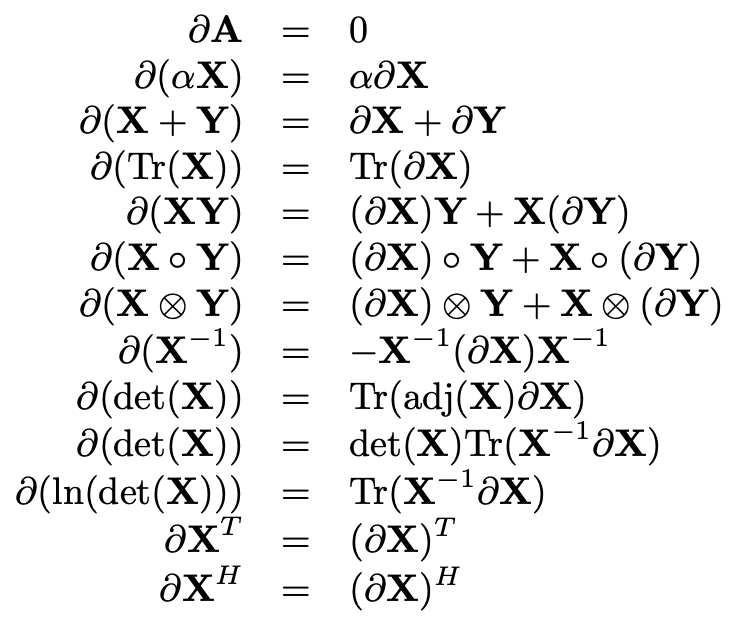
\includegraphics[width=.7\columnwidth]{src/matrix_deriv.png}

\subsection*{Matrices}

Cauchy-Schwarz: $\mathbf a^\top\mathbf b \leq \|\mathbf a\|_2\|\mathbf b\|_2$

Norms: $\mathbf w^\top\mathbf w=\|\mathbf w\|_2^2$, $\mathbf w^\top\text{sgn}(\mathbf w)=\sum_i |x_i|=\|\mathbf w \|_1$

Traces: $\text{Tr}(A+B)=\text{Tr}(A)+\text{Tr}(B)$, $\text{Tr}(AB)=\text{Tr}(BA)$, $\mathbf{a}^T \mathbf a = \text{Tr}(\mathbf{aa}^T)$, $\mathbf x^T\mathbf M\mathbf x=\text{Tr}(\mathbf x^T\mathbf M\mathbf x)$, $\mathbf x^T\mathbf y = \text{Tr}(\mathbf{yx}^T)$, if $\mathbf A$ s.p.d then $\text{Tr}(\mathbf A)\geq 0$.

Vector projection $\mathbf a$ to $\mathbf b$: $\frac{\mathbf a^\top \mathbf b}{\|\mathbf b\|^2}\mathbf b$

\iffalse
\subsection*{Parametric vs. Nonparametric}
\textbf{Parametric}: have finite set of parameters. 
e.g. linear regression, linear perceptron\\
\textbf{Nonparametric}: grow in complexity with the size of the data, more expressive.
e.g. k-NN
\fi
%\section*{Regression}
\textbf{SVD:}$\X=\mathbf{U}\Sigma\mathbf{V}^T$\\
\textbf{Model}:
$y=w_0 + \sum_{j=1}^d\mathbf{X_j} w_j$, $y\subset{\mathbb{R}}$\\
Introduce $X_0=1$ and rewrite\\
$y=\mathbf{X} \w \quad \mathbf{X}\in\mathbb{R}^{d\times n},  w \in \mathbb{R}^{d+1}$\\
Gau.noise$\epsilon \sim \mathcal{N}(0,\sigma^2)$;$y\sim \N(||\X||_2,\sigma^2)$\\
$\E[y|\X]=X^T w$
depending linearly on $(1,\x_1,...,\x_d)$;
$\hat{y}=\mathbf{X}\hat{ w}+\epsilon$\\
$\hat{ w} \sim \mathcal{N}( w, (\mathbf{X}^T\mathbf{X})^{-1}\sigma^2) $ and\\
$p(Y|X, w, \sigma) \sim \mathcal{N}(Y|X^T w, \sigma^2)$

% A Regression has Optimum:\\
% $f^*(x) = \mathbb{E}_Y[Y|X=x]$


\subsection*{Ordinary Least Squares}
$\hat R(w)=\sum_{i=1}^n(y_i-\w^T x_i)^2=||\y-\X\w||^2$\\
% $X\in\mathbb{R}^{n\times(d+1)}, y\in\mathbb{R}^n,   w\in\mathbb{R}^{d+1}$\\
$\hat \w = (\X^T\X)^{-1}\X^T\y=\mathbf{V}\Sigma^{-1}\mathbf{U}^T\y$\\
$\w^*$ \textbf{exists:} $\X^T\X$ invertible$\Leftrightarrow \X$full rank $\Leftrightarrow \X$ full column rank.
$\E_{\epsilon |\X}[\hat\w]=w\Rightarrow$ unbiased, $\V(\hat \w)=\sigma^2(\X^T\X)^{-1}$;
orth. projection with lowest variance of all unbiased estimates.\\
\textbf{Prediction:} $\hat{y}{=}\mathbf{X}\hat{ w}{=}\mathbf{X}(\mathbf{X}^T\mathbf{X})^{-1}\mathbf{X}^{T}\mathbf{y}$
\subsection*{Ridge Regression ($L^2$ penalty)}
$\hat R_{ridge}(w)=\sum_{i=1}^n(y_i-\w^T x_i)^2+\lambda\w^T\w=||\y-\X\w||^2+\lambda||\w||^2$;
$\hat \w_{ridge}(\lambda)=(\X^T\X+\lambda \I_d)^{-1}\X^T\y=\mathbf{V}(\Sigma^2+\lambda \I)^{-1}\Sigma\mathbf{U}^T\y$\\
$\E_{\epsilon |\X}[\hat\w_{r}]=(\X^T\X+\lambda\I)^{-1}(\X^T\X)\w$;biased
$\V(\hat \w_{ridge})=\sigma^2(\X^T\X+\lambda\I)^{-1}(\X^T\X)$\\$[(\X^T\X+\lambda\I)^{-1}]^T$;
$\V(\hat \w)\geq\V(\hat \w_{ridge})$;
%Bayes: $Y|(X, w)\sim\N(x^T w,\sigma^2\I)$;\\
%prior: $ w\sim\N(0,\frac{\sigma^2}{\lambda}\I)$;
$\hat R_{ridge}(w)$ convex $\Leftrightarrow$ Hessian $D^2\hat R_{ridge}(w)$ positive semi definite;
strictly convex; always unique sol; $\lambda \w^T\w$  biases sol. towards origin; shrinks the low variance components, $\Sigma_{jj}=d_{jj}\Rightarrow d_{jj}^{-1}\geq \frac{d_{jj}}{d_{jj}^2}+\lambda; \forall \lambda >0$

\subsection*{Lasso ($L^1$ penalty)}
$\hat R_{lasso}(\w) = ||\y-\X\w||^2+\lambda|| w||_1$\\
no closed form; sparse solutions $\rightarrow$ better generalization than ridge; convex;diamond

% \iffalse
% \subsection*{Bayesian Linear Regression}
% \textbf{Setting:} Define a prior over $ w$.\\
% \textbf{e.g. Ridge:} Assume $ w$ distributed as:\\
% $p( w|\bm{\bm{\Lambda}}){=}\mathcal{N}( w|\mathbf{0},\frac{\sigma^2}{\lambda}\mathbb{I}) \propto \mathrm{exp}(-\frac{\lambda}{2\sigma^2} w^T w)$\\
% For $\bm{\Lambda}=\frac{\sigma^2}{\lambda}\mathbb{I}$. Linear for $\sigma=1$.

% Then, given observed $\mathbf{X},\mathbf{y}$, use Bayes' theorem to find the posterior\\
% $p( w|\mathbf{X},\mathbf{y}, \bm{\Lambda}, \sigma) = \mathcal{N}(\mu_{ w}, \Sigma_{ w})$\\
% $\mu_ w = \sigma^2(\mathbf{X}^T\mathbf{X} +\sigma^2\bm{\Lambda})^{-1}\mathbf{X}^T\mathbf{y}$\\
% $\Sigma_ w = \sigma^2(\mathbf{X}^T\mathbf{X} +\sigma^2\bm{\Lambda})^{-1}$
% \fi

\subsection*{Nonlinear Regression}
basis expansion
\textbf{Idea:} Feature space transformation\\
Model: $\mathbf{Y}=f(\mathbf{X})=\sum_{i=1}^d\w_i \phi_i(\x)$\\
Transformation $\phi_i(\mathbf{X}):\mathbb{R}^d \rightarrow \mathbb{R}$

% \iffalse
% \section*{Bias-Variance tradeoff}
% Bias($\hat{f}$)$=\mathbb{E}[\hat{f}]-f$\\
% Var($\hat{f}$)$=\mathbb{E}[(\hat{f}-\mathbb{E}[\hat{f}])^2]$\\
% $|\mathcal{Z}|\downarrow \quad|\mathcal{F}|\uparrow\quad\Rightarrow\quad\mathrm{Var}\uparrow\quad\mathrm{Bias}\downarrow $\\
% $|\mathcal{Z}|\uparrow \quad|\mathcal{F}|\downarrow\quad\Rightarrow\quad\mathrm{Var}\downarrow\quad\mathrm{Bias}\uparrow $

% \subsection*{Squared Error Decomposition}
% $\mathbb{E}_D\mathbb{E}_{X,Y}[(\hat{f}(X)-Y)^2]=$\\
% $\mathbb{E}_{X,Y}[(\mathbb{E}_{Y|X}[Y]-Y)^2]$ (noise$^2$)\\
% $+\mathbb{E}_X\mathbb{E}_D[(\hat{f}_D(X)-\mathbb{E}_D[\hat{f}(X)])^2]$ (var.)\\
% $+\mathbb{E}_X[(\mathbb{E}_D[\hat{f}_D(X)]-\mathbb{E}_{Y|X}[Y])^2]$ (bias$^2$)\\
% With $\mathbb{E}_{Y|X}[Y]$ the expected label and $\mathbb{E}_{D}[\hat{f}(X)$ the expected classifier.
% \fi
%\section*{Model Selection}
\subsection*{K-Fold Cross Validation}
split training set:$K=\min\{\sqrt{n},10\}$\\
$\mathcal{Z}=\bigsqcup^{K}_{i=1}\mathcal{Z}_i $;
% with map $\kappa:\{1,\cdots, n\} \rightarrow\{, \cdots, K\}$
$|\mathcal{Z}_k|\approx n\frac{K-1}{K}$ \# of samples\\
%Learning:\\
$\hat{f}^{-\nu}(x){=}
\argmin_{f\in\mathcal{F}}\frac{\sum_{i\not\in\mathcal{Z}_\nu}(y_i-f(x_i))^2}{|\mathcal{Z}\setminus\mathcal{Z}_{\nu}|}$\\
%Validation:\\
$\hat{R}^{cv} = \frac{1}{n}\sum_{i\leq n}(y_i-\hat{f}^{-\kappa(i)}(x_i))^2$\\
Underfits because smaller dataset.\\
\textbf{Leave-one-out:} $K=n$ (unbiased but var can be large from corr. datasets)

% \subsection*{Bootstrapping}
% Bootstrap samples: $\mathcal{Z}^*=\{\mathcal{Z}_1^*, \cdots\mathcal{Z}_B^*\}$, of same size as original, drawn with replacement.
% The chance of a sample to have appeared in the bootstrap is:\\
% $1-(1-\frac{1}{n})\stackrel{n\to\infty}{\to} 1-\frac{1}{e}\approx 0.632$. So if we compute the ERM on $\mathcal{Z}$ we could get 63\% accuracy by memorization. Over-confident!\\
% \textbf{Leave-one-out}: compensates by computing the ERM where no memorization was for specific sample. E.g., for classification, like cross-validation:\\
% $\hat{\mathcal{R}}(S(\mathcal{Z}))=\frac{1}{B}\sum_{b=1}^B\sum_{z_i\not\in\mathcal{Z}^{*b}}\frac{\mathbb{I}_{c(x_i)\neq y_i}}{B-\lvert\mathcal{Z}^{*b}\rvert}$

% \subsection*{Jackknife}
% Estimate of an estimator $\hat{S}_n$'s Bias.\\
% $\hat{S}^{JK}=\hat{S}_n-\mathrm{bias}^{JK}$ is JK Estimator.\\
% $\mathrm{bias}^{JK}{=}(n{-}1)(\tilde{S}_n{-}\hat{S}_m)$\\
% $\tilde{S}_n{=}\frac{1}{n}\sum_{i=1}^n\hat{S}_{n{-}1}^{-i}$ avg. LOO Estimator.
% Debiased est. can have big variance!\\
% \textbf{Bootstrap debiased}\\ $\bar{S}{=}2\hat{S}{-}\frac{1}{B}\sum_b\hat{S}^*(b)$


%\section*{Classification}
% $w^* = \underset{w}{\operatorname{argmin}} ~ l(w;x_i,y_i)$
\subsection*{Metrics $n = n_+ + n_- = p_+ + p_-$}
$n_+ = \text{TP} + \text{FN}$, $n_- = \text{TN} + \text{FP}$, $p_+ = \text{TP} + \text{FP}$, $p_- = \text{FN} + \text{TN}$
Accuracy: $\frac{\text{TP}+\text{TN}}{n}$; \\
Precision: $\frac{\text{TP}}{\text{TP}+\text{FP}}$
Recall/TPR: $\frac{\text{TP}}{n_+}$; \\
FPR: $ \frac{\text{FP}}{n_-}$;
F1:$\frac{2TP}{2TP+FP+FN}=\frac{2}{\frac{1}{\text{Precision}}+\frac{1}{\text{Recall}}}$\\
ROC Curve: $y = $TPR, $x = $FPR; $A1 \succ A2$ in ROC $\Leftrightarrow A1 \succ A2$ in precision/recall curve
% $F_1=2\frac{\text{pre}*\text{rec}}{\text{pre}+\text{rec}}$\\
\subsection*{Loss}
$l_{0/1}(\w;\x_i,y_i)=1:\; \text{if}\;y_i\neq \text{sign}(\w^T\x_i), 0:\text{else}$\\
$l_{P}(\w;\x_i,y_i)=\max(0,-y_i\w^Tx_i)$, conv.surrogate for $l_{0/1}$;\\
$l_{H}(\w;\x_i,y_i)=\max(0,1-y_i\w^T\x_i)$
\subsection*{Perceptron}
SGD on $l_P$ with $\eta=1$;
$\nabla_w l_P(w;y_i,x_i) = 
\begin{cases}
    0 &\text{if } y_i w^T x_i \geq 0\\
    -y_i x_i &\text{otherwise}
\end{cases}$ \\
% \subsection*{Linear Classifier}
% % optimal for Gaussian with equal cov. Stat. simplicity \& comput. efficiency.
% $g(x)=a^T\tilde{x}\quad a=(w_0,w)^T, \tilde{x}=(1,x)^T$\\
% $a^T\tilde{x}_i>0 \Rightarrow y_i=1, a^T\tilde{x}_i<0 \Rightarrow y_i=2$\\
% Normalization: $\tilde{x}_i\rightarrow-\tilde{x}_i$ if $y_i=2$
% Find $a$: $a^T\tilde{x}_i>0,\forall i$

% \subsection*{Perceptron Criterion}
% $J_P(a)=\sum_{\tilde{x}\in\mathcal{X}^\text{msc}}(-a^T\tilde{x})$,\\
% $\mathcal{X}^\text{msc}$: set of misclassified samples.\\
% $\Rightarrow a(k+1)=a(k)+\eta(k) \sum_{\tilde{x}\in\mathcal{X}^\text{msc}} \tilde{x}$\\
% Converges if data separable.\\
% Single sample perceptron: $(k++)\mod n$\\
% $a(k+1)=a(k)+\tilde{x}^k$ (misclassified).

%\subsection*{Fisher's Linear Discriminant Analysis}
%Maximize distance of the means of the projected classes to find projection plane separating them best.\\
%proj mean: $\tilde{m}_{\alpha}{=}\frac{1}{n_{\alpha}}\sum_{x\in\mathcal{X}_{\alpha}}w^Tx{=}w^Tm_{\alpha}$\\
%Dist of proj means: $|w^T(m_1-m_2)|$
%Classes proj. cov: $\tilde{\Sigma}_1{+}\tilde{\Sigma}_2{=}w^T(\Sigma_1{+}\Sigma_2)w$\\
%Fishers Criterion:\\
%$J(w)=\frac{||m_1-m_2||^2}{\tilde{\Sigma}_1{+}\tilde{\Sigma}_2}=\frac{w^T(m_1-m_2)(m_1-m_2)^Tw}{w^T(\Sigma_1{+}\Sigma_2)w}$
%Fishers Crit for Multiple Classes:\\
%$J(W)=\frac{|W^T\Sigma_BW|}{W^T\Sigma_WW}$\\
%$\Sigma_B=\sum_{i=1}^kn_k(m_k-m)(m_k-m)^T$\\
%$\Sigma_W=\sum_{i=1}^k\sum_{x\in \mathcal{D}_i}(x-m_i)(x-m_i)^T$

% \textbf{LDA for Multiclasses}: 
% Reformulate as $(k-1)$ ``class $\alpha$ - not class $\alpha$'' dichotomies. But some area are ambiguous

\subsection*{Support Vector Machine (SVM)}
$\nabla_w l_H(w;y,x) = 
\begin{cases}
    0 &\text{if } y_i w^T x_i \geq 1\\
    -y_i x_i &\text{otherwise}
\end{cases}$\\
$w^* = \argmin_\w ~\frac{1}{n}\sum_{i=1}^nl_H(w;x_i,y_i)+\lambda||w||_2^2$\\ For L1-SVM (feature selection) use $||w||_1$ 
save learning rate: $\eta_t=\frac{1}{\lambda t}$
% Generalize Perceptron with margin $m$ and kernel. Find plane that $\max  m$ s.t.:\\
% $z_ig(\mathbf{y})=z_i(\mathbf{w}^T\mathbf{y}+w_0)\geq m,\forall \mathbf{y}_i \in \mathcal{Y}$\\
% $z_i \in \{-1,+1\}\quad \mathbf{y_i} = \phi(\mathbf{x_i})$\\
% \textbf{Support Vectors:} $\mathbf{y}_i$ with $z_ig(\mathbf{y}_i)=m$
% Functional Margin Problem:\\
% minimizes $||\mathbf{w}||$ for $m{=}1$: 
% $L(\mathbf{w}, w_0, \mathbf{\alpha}) {=}$\\
% $=\frac{1}{2}\mathbf{w}^T\mathbf{w}{-}\sum_{i=1}^n\alpha_i[z_i(\mathbf{w}^T\mathbf{y}_i{}+w_0){-}1]$\\
% where $\alpha_i$ are Lagrange multipliers.
% $\frac{\partial L}{\partial w} {=} 0$\\ $\frac{\partial L}{\partial w_0} {=} 0 \Rightarrow \mathbf{w}=\sum_{i=1}^n\alpha_iz_i\mathbf{y_i} \quad 0=\sum_{i=1}^n\alpha_iz_i$\\
% %Replacing these in $L(\mathbf{w}, w_0, \mathbf{\alpha})$ we get\\
% $\tilde{L}(\mathbf{\alpha}){=}\sum_{i=1}^n\alpha_i{-}\frac{1}{2}\sum_{i,j=1}^n\alpha_i\alpha_jz_iz_j\mathbf{y_i}^T\mathbf{y_j}$
% max
% with$\alpha_i\geq0\quad$  $\quad\sum_{i=1}^n\alpha_iz_i=0$; Dual\\
% optimal hyperplane:
% $\mathbf{w^*}=\sum_{i=1}^n\alpha_i^*z_i\mathbf{y_i}$\\
% $ w_0^*{=}{-}\frac{1}{2}(\mathrm{min}_{z_i=1}\mathbf{w^*}^T\mathbf{y_i}{+}\mathrm{max}_{z_i=-1}\mathbf{w^*}^T\mathbf{y_i})$\\
% Only Support Vectors ($\alpha_i\not=0$) contribute to the evaluation.\\
% Optimal Margin: $\mathbf{w}^T\mathbf{w}=\sum_{i\in SV}\alpha_i^*$\\
% Discrim.: $g^*(\mathbf{y}){=}\sum_{i\in SV}z_i\alpha_i\mathbf{y_i}^T\mathbf{y}{+}w^*_0$\\
% $\mathrm{class} = \mathrm{sign(\mathbf{y}^T\mathbf{w}^*+w_0^*)}$

% \subsection*{Soft Margin SVM}
% Introduce slack to relax constraints\\
% $z_i(\mathbf{w}^T\mathbf{y}_i+w_0)\geq m(1-\xi_i)$; $\xi_i \geq 0$\\
% $L(\mathbf{w}, w_0,\mathbf{\xi}, \mathbf{\alpha}, \mathbf{\beta}) {=}\frac{1}{2}\mathbf{w}^T\mathbf{w}+C\sum_{i=1}^n\xi_i-$\\
% ${-}\sum_{i=1}^n\alpha_i[z_i(\mathbf{w}^T\mathbf{y}_i{+}w_0){-}1{+}\xi_i]$\\
% ${-}\sum_{i=1}^n\beta_i\xi_i$; $\, \frac{\partial L}{\partial\xi_i}= C-\alpha_i-\beta_i=0$\\
% $C\downarrow\Rightarrow m\downarrow\wedge\mathrm{constrain}\, \mathrm{violation}\downarrow$ \\
% Dual constraints:
% $C \geq \alpha_i \geq 0$

% \subsection*{Non-Linear SVM}
% Use kernel in discriminant funct: $g(\mathbf{x})=\sum_{i,j=1}^n\alpha_i\alpha_jz_iz_jK(\mathbf{x_i},\mathbf{x})$\\
% E.g solve the XOR Problem with:
% $K(x,y)=(1+x_1y_1+x_2y_2)^2$

% \subsection*{Multiclass SVM}
% $\forall$class $z\in\{1,2,\cdots,M\}$ introduce $\mathbf{w}_z$ and define the margin $m$ s.t.:  $\min_{\mathbf{w_z}}\frac{1}{2}\sum_{z=1}^M\mathbf{w}_z^T\mathbf{w}_z$\\
% $(\mathbf{w}_{z_i}^T\mathbf{y}_i+w_{z_i,0})-\max_{z\not=Z_i}(\mathbf{w}_z^T\mathbf{y}_i+w_{z,0})\geq m, \forall{\mathbf{y}_i\in \mathcal{Y}}$

% \subsection*{Structured SVM}
% Each sample $\mathbf{y}$ is assigned to a structured output label $z$\\
% Output Space Representation:\\
% joint feature map: $\mathbf{\psi}(z,\mathbf{y})$\\
% Scoring function: $f_{\mathbf{w}}(z,\mathbf{y})=\mathbf{w}^T\mathbf{\psi(z, \mathbf{y})}$\\
% Classify: $\hat{z}=h(\mathbf{y})\argmax_{z\in\mathcal{K}}f_{\mathbf{w}(z, \mathbf{y})}$
\subsection*{Multi class}
$l_{MC-H}(w^{(1)},...,w^{(c)};x,y) =
\max (0,1+\max_{j\in\{1,\cdots,y-1,y+1,\cdots,c\}} w^{(j)T} x - w^{(y)T} x)$
%\section*{Feature selection}
\subsection*{Greedy feature selection}
slow, high computational cost;
applies to any prediction method
\subsubsection*{Forward}
start with 0 feat. add best feat as long as error decreases.
\textbf{Problem:} 1 feature $\Rightarrow$ 50\% error rate;
usually faster
\subsubsection*{Backward}
start with all feat. remove worst feat as long as error decreases.
Can handle dependent feat.
\subsection*{L1 as surrogate for L0}
fast,(training and feat selection happen jointly);
only works for linear models
%\section*{Kernels $K(\mathbf{x}, \mathbf{x'}) {=} \phi(\mathbf{x})^T\phi(\mathbf{x'})$}
Similarity based reasoning\\
Gram Matrix $K{=}K(\mathbf{x}_i, \mathbf{x}_j), 1{\leq} i,j{\leq} n$\\
sym. p.s.d.(all EV $\geq$ 0); Engineering:\\
$K_1(\mathbf{x}, \mathbf{x'})K_2(\mathbf{x}, \mathbf{x'})$; 
$\alpha K_1(\mathbf{x}, \mathbf{x'})+\beta K_2(\mathbf{x}, \mathbf{x'})$\\
$\phi:\mathcal{X}{\rightarrow}\mathcal{X},\,\,K(\phi(\mathbf{x}), \phi(\mathbf{x'}))$; $p(h|\mathbf{x})p(h'|\mathbf{x'})$\\ 
$h: \mathrm{poly/exp},\,\, h(K(\mathbf{x}, \mathbf{x'}))$;$ \, f(\mathbf{x})K(\mathbf{x},\mathbf{x'})f(\mathbf{x'})$

lin/poly: $\mathbf{x}^T\mathbf{x'}$; $(\mathbf{x}^T\mathbf{x'}{+}1)^p$;
$\mathrm{dim}=\binom{n+p}{p}$\\
RBF(Gauss): $\exp(-||\mathbf{x}{-}\mathbf{x'}||_2^2/h^2)$\\
lapl: $\exp(-||\mathbf{x}{-}\mathbf{x'}||_1/h)$, $h\uparrow$: regularizat.\\
Sigmoid:$\mathrm{tanh}(\alpha\mathbf{x}^T\mathbf{x'}+c)$\\
not p.s-d eg: $\mathbf{x}{=}[1,-1], \mathbf{x'}{=}[-1,2]$

\subsection*{Reformulating the perceptron}
Ansatz: $w^* \in \operatorname{span}(X) \Rightarrow w = \sum_{j=1}^n \alpha_j y_j x_j$\\
$\alpha^*= \argmin_{\alpha} \frac{1}{n} \sum_{i=1}^n \max(0,$\\$- \sum_{j=1}^n \alpha_j y_i y_j x_i^T x_j)$

\subsection*{Kernelized perceptron and SVM}
Use $\alpha^T k_i$ instead of $w^T x_i$,\\
use $\alpha^T D_y K D_y \alpha$ instead of $||w||_2^2$\\ 
$k_i=[y_1 k(x_i,x_1), ..., y_n k(x_i,x_n)]$;\\
$D_y = \text{diag}(y)$\\
Prediction: $f(\hat{x}) = \operatorname{sign}(\sum_{i=1}^n \alpha_i y_i k(x_i, \hat{x}))$

\subsection*{Kernelized linear regression (KLR)}
Ansatz: $w^*=\sum_{i = 1}^n \alpha_i x$\\
$\alpha^*= \argmin_{\alpha}\frac{1}{n} ||\alpha^T K - y||_2^2 + \lambda \alpha^T K \alpha \\= (K+\lambda I)^{-1} y$\\
Prediction: $f(\hat{x}) = \sum \limits_{i=1}^n \alpha_i k(x_i,\hat{x})$

% TODO commented this out because there were errors
%\section*{Neural network}
Parameterize feature map: $\phi(x,\theta)$ instead of $\phi(x)$, usually: $\phi(x,\theta) = \varphi(\theta^T x) = \varphi(z)$\\
$\Rightarrow w^* = \underset{w, \theta}{\operatorname{argmin}} \sum_{i=1}^n l(y_i; \sum_{j=1}^m w_j \phi(x_i, \theta_j))$

\subsection*{Activation functions}
Sigmoid: $\sigma(z)=\frac{1}{1+e^{-z}}$,\\
$\sigma'(z) = (1 - \sigma(z))\cdot\sigma(z)$\\
Tanh: $\varphi(z) = tanh(z) = \frac{exp(z)-exp(-z)}{exp(z)+exp(-z)}$\\
ReLu:  $\varphi(z) = max(z,0)$

\subsection*{Predict: forward propagation}
$v^{(0)} = x$; for $l = 1,...,L-1$:
$v^{(l)} = \varphi(z^{(l)})$; $z^{(l)} = W^{(l)}v^{(l-1)}$;
$f = W^{(L)}v^{(L-1)}$\\
Predict $f$ for regression, $\operatorname{sign}(f)$ for class.

\subsection*{Compute gradient: backpropagation}
Output layer: 
$\delta_j = l_j'(f_j)$,
$\frac{\partial}{\partial w_{j,i}} = \delta_j v_i$\\
Hidden layer $l=L-1,...,1$:\\
$\delta_j = \varphi'(z_j) \cdot \sum_{i\in Layer_{l+1}} w_{i,j}\delta_i$,
$\frac{\partial}{\partial w_{j,i}} = \delta_j v_i$

\subsection*{Learning with momentum}
$a \leftarrow m \cdot a + \eta_t \nabla_W l(W;y,x)$; $W \leftarrow W - a$
%\section*{Clustering}
\subsection*{k-mean}

$\hat{R}(\mu) = \sum_{i=1}^n \underset{j\in\{1,...k\}}{\operatorname{min}}||x_i-\mu_j||_2^2$\\
$\hat{\mu} =  \argmin_{\mu} ~ \hat{R}(\mu)$;non-convex, NP-hard \\
\subsubsection*{Algorithm (Lloyd's heuristic)}
Init: $\mu^{(0)}$; while not converged:\\
$z_i^{(t)}=\argmin_{j \in \{1,...,k\}}||\x_i-\mu_j^{(t-1)}||_2^2$;
$\mu_j^{(t)}=\frac{1}{|\{i:z_i^{(t)}=j\}|}\sum_{i:z_i^{(t)}=j}x_i$; $O(nkd)$per iter
% Choose starting centers, assign points to closest center, update centers to mean of each cluster, repeat

%\subsection*{k-mean++}
%- Start with random data point as center\\
%- Add centers 2 to k randomly, proportionally to squared distance to closest selected center\\
%for $j=2$ to $k$:
%$i_j$ sampled with prob.\\
%$P(i_j=i) = \frac{1}{z} \underset{1\leq l<j}{min}||x_i-\mu_l||_2^2$; $\mu_j \leftarrow x_{i_j}$
%\section*{Dimension reduction}
\subsection*{PCA}
$D\subset \mathbb{R}^d$; $\mu = \frac{1}{n}\sum_{i=1}^nx_i=0$; 
$\Sigma = \frac{1}{n}\sum_{i=1}^n x_i x_i^T$\\
$(W,z_1,...,z_n) = \operatorname{argmin} \sum_{i=1}^n||W z_i - x_i||_2^2$;\\
$W = (v_1|...|v_k) \in \mathbb{R}^{d \times k}$ ortho; $z_i = W^T x_i$ \\ 
$v_i$ eigenvec of $\Sigma$

\subsection*{Kernel PCA}
$\alpha^{(1)},...,\alpha^{(k)}\in \mathbb{R}^n$, $\alpha^{(i)} = \frac{1}{\sqrt{\lambda_i}}v_i$, $K = \sum_{i=1}^n \lambda_i v_i v_i^T$, $\lambda_1 \geq ... \geq \lambda_d \geq 0$\\
New p: $z = f(\x) = \sum_{j=1}^n\alpha_j^{(i)}k(\x,x_j)$; $z\in \R^k$

\subsection*{Autoencoders}
Find identity function: $x \approx f(x;\theta)$\\
$f(x;\theta) = f_{decode}(f_{encode}(x;\theta_{encode});\theta_{decode})$
%\section*{Probability modeling}
Find $h:X\rightarrow Y$ that min. pred. error: 
$R(h) = \int P(x,y)l(y;h(x)) \partial yx \partial y = \mathbb{E}_{x,y}[l(y;h(x))]$

\subsection*{For least squares regression}
Best $h$: $h^*(x) = \mathbb{E}[Y|X=x]$ \\
Pred.: $\hat{y} = \hat{\mathbb{E}}[Y|X=\hat{x}] = \int \hat{P}(y|X=\hat{x}) y \partial y$

\subsection*{MLE}
$\theta^* = \underset{\theta}{\operatorname{argmax}} ~ \hat{P}(y_1,...,y_n|x_1,...,x_n,\theta)$\\
lin. + Gauss: $y_i = w^T x_i + \varepsilon_i, \varepsilon_i \sim \mathcal{N}(0, \sigma^2)$\\
i.e. $y_i \sim \mathcal{N}(w^T x_i, \sigma^2)$, With MLE (use\\ $\operatorname{argmin} ~ - \operatorname{log}$): $w^* = \underset{w}{\operatorname{argmin}} \sum (y_i-w^Tx_i)^2$

\subsection*{Bias/Variance/Noise}
Pred error = $Bias^2 + Variance + Noise$

\subsection*{MAP}
Assume bias on parameters, e.g. $w_i \in \mathcal{N}(0, \beta^2)$;
Bay.: $P(w|x,y) = \frac{P(w|x) P(y|x,w)}{P(y|x)} = \frac{P(w) P(y|x,w)}{P(y|x)}$
\subsection*{Logistic regression}
sigmoid:$\sigma(w^Tx) = \frac{1}{1+exp(-w^Tx)}$\\
$P(y|x,w) = Ber(y; \sigma(w^Tx)) = \frac{1}{1+exp(-y w^T x)}$\\
\textbf{CLF}: Use $P(y|x,w)$, predict most likely class label.
\subsubsection*{MLE}
$\underset{w}{\operatorname{argmax}} ~ P(y_{1:n}|w,x_{1:n})\\
w^* = \underset{w}{\operatorname{argmin}} \sum_{i=1}^n log(1+exp(-y_i w^T x_i))$\\
\textbf{SGD}: $w = w + \eta_t y x \hat{P}(Y = -y|w,x)$\\
$\hat{P}(Y = -y|w,x) = \frac{1}{1+exp(yw^Tx)}$
\subsubsection*{MAP} Gauss. prior: $||w||_2^2$, Lap. prior: $||w||_1$\\
\textbf{SGD}: $w = w (1-2\lambda \eta_t) + \eta_t y x \hat{P}(Y = -y|w,x)$
%\section*{Bayesian decision theory}
- Cond. dist. over labels $P(y|x)$\\
- Set of actions $\mathcal{A}$\\
- Cost function $C:Y\times \mathcal{A} \rightarrow \mathbb{R}$\\
$a^* = \underset{a \in \mathcal{A}}{\operatorname{argmin}} ~ \mathbb{E}[C(y,a)|x]$\\
\subsubsection*{Classification} $C(y,a) = [y \not = a]$; asymmetric: \\
$C(y,a) =
 \begin{cases}
 	c_{FP} \text{ , if $y=-1$, $a=+1$}\\
		c_{FN} \text{ , if $y=+1$, $a=-1$}\\
		0 \text{ , otherwise}
 \end{cases}$
\subsubsection*{Regression}  $C(y,a) = (y-a)^2$; asymmetric: $C(y,a) = c_1 \max(y-a,0) + c_2 \max(a-y,0)$
% E.g. $y \in \{-1,+1\}$, pred$+$if $c_+ < c_-$,\\
% $c_+ = \mathbb{E}(C(y, +1)|x) = P(y = 1|x) \cdot 0 + P(y = -1|x) \cdot c_{FP}$, $c_-$ likewise

%\subsection*{Optimal decision for logistic regression}
%$a^* = \underset{y}{argmax} \hat{P}(y|x) = sign(w^T x)$

% \subsection*{Example: logistic regression}
% \begin{itemize}
% 	 Est. cond. dist: $P(y|x,w) = Ber(\sigma(w^Tx))$
% 	 Action set: $\mathcal{A} = \{ +1, -1\}$
% 	 Cost function: $C(y,a) = [y \not = a]$ \\ 
% 	$= \left \{ 
% 		\begin{array}{lr}
% 			1 \text{ , if } y \not = a\\
% 			0 \text{ , otherwise}
% 		\end{array}
% 		$
% \end{itemize}
% $a^* = \underset{a \in \mathcal{A}}{\operatorname{argmin}} \mathbb{E}_y[C(y,a)|x]$\\
% $= \underset{a \in \mathcal{A}}{\operatorname{argmin}} P(y=1|x,w)[a=1] + P(Y=-1|x,w)[a=+1]$\\
% $= \underset{a \in \mathcal{A}}{\operatorname{argmin}} P(y \not = a | x,w) = \underset{a \in \mathcal{A}}{\operatorname{argmin}} \frac{1}{1+exp(aw^Tx)}$\\
% $=\underset{a \in \mathcal{A}}{\operatorname{argmax}} (1 + exp(aw^Tx))$
% $=\underset{a \in \mathcal{A}}{\operatorname{argmax}} (aw^Tx)$\\
% $= sign (w^Tx)$

%\subsection*{Example: Asymmetric costs}
%	 Est. cond. dist: $\hat{P}(y|x,w) = Ber(\sigma(w^Tx))$
%	 Action set: $\mathcal{A} = \{ +1, -1\}$
%	 Cost function: $C(y,a) =
%	 \begin{cases}
%	 	c_{FP} \text{ , if $y=-1$ and $y=+1$}\\
%			c_{FN} \text{ , if $y=+1$ and $y=-1$}\\
%			0 \text{ , otherwise}
%	 \end{cases}
%		$
%The action that minimizes the expected cost is:\\
%$C_+ = \mathbb{E}_y[C(y,+1)|x] = P(y=+1|x) \cdot 0 + (P(y=-1)|x) \cdot c_{FP}$\\
%$C_- = \mathbb{E}_y[C(y,-1)|x] = P(y=+1|x) \cdot c_{FN} + P(y=-1|x) \cdot 0$\\
%Predict +1 if $C_+ \leq C_- \Leftrightarrow P(y=+1|x) \geq \frac{c_{FP}}{c_{FP} + c_{FN}}$

%\subsection*{Doubtful logistic regression}
%	 Est. cond. distr.: $\hat{P}(y|x) = Ber(y;\sigma(\hat{w}^Tx))$\\
%	 Action set: $\mathcal{A} = \{ +1, -1, D\}$;  Cost function:\\
%	 $C(y,a) = \begin{cases}
%			[y \neq a] &\text{if } a \in \{+1,-1\}\\
%			c &\text{if } a = D
%       \end{cases}$\\
%The action that minimizes the expected cost\\
%$a^* = y \text{ if } \hat{P}(y|x) \geq 1-c\text{, D otherwise}$
%$a^* = \begin{cases}
%		y &\hat{P}(y|x) \geq 1-c\\
%		D &\text{otherwise}
%	   \end{cases}
%$

%\subsection*{Least squares regression}
%	 Est. cond. distr.: $\hat{P}(y|x,w) = \mathcal{N}(y;w^Tx, \sigma^2)$\\
% $\mathcal{A} = \mathbb{R}$; $C(y,a) = (y-a)^2$\\
%The action that minimizes the expected cost\\
%$a^* = \mathbb{E}_y[y|x] = \int \hat{P}(y | x) \partial y = \hat{w}^Tx$

%\subsection*{Asymmetric cost for regression}
%	 Est. cond. distr.: $\hat{P}(y|x) = \mathcal{N}(\hat{y};\hat{w}^Tx, \sigma^2)$\\
%	 $\mathcal{A} = \mathbb{R}$; $C(y,a) = c_1 \max(y-a,0) + c_2 \max(a-y,0)$
%Action that minimizes the expected cost:\\
%$a^* = \hat{w}^Tx + \sigma \Phi^{-1} (\frac{c_1}{c_1 + c_2})$, $\Phi$: Gaussian CDF\\
%$\frac{\partial}{\partial a}$\\
%$\frac{\partial}{\partial a} \mathbb{E}_y[C(y,a)|x] = \int_{-\infty}^{\infty} C(y,a) P(y | x) dy \overset{!}{=} 0$\\
%$= -c_1 \int_{a}^{\infty} P(y | x) dy + c_2 \int_{-\infty}^{a} P(y | x) dy$\\
%$= -c_1 [1-\phi(a; w^Tx, \sigma^2)] + c_2 \phi(a; w^Tx, \sigma^2)$\\
%$\phi(a; w^Tx, \sigma^2) = \frac{c_1}{c_1 + c_2}$\\
%using $\phi(u;v,w) = \phi((u-v)/\sqrt{w};0,1)$ and applying inverse CDF of std. ND $\phi^{-1}$ we get\\
%$a^* = w^Tx + \sigma\phi^{-1} (\frac{c_1}{c_1 + c_2})$
%\section*{Generative modeling}
estimate joint: $P(y,\x)$; can derive cond from joint;
1. generate class labels: $P{(y)}$ \textbf{MLE};
2. generate feat given class: $P(\x|y)$ \textbf{MLE};
3. obtain pred: $P(y|\x)=\frac{P(y)P(\x|y)}{Z}$,
$Z=P(\x)=\sum_yP(\x,y)=\sum_yP(y)P(\x|y)$ \textbf{MAP};
\subsection*{Discriminative}
estimate cond: $P(y|\x)$; not modeling $P(\x)$;
no outlier detection

\subsection*{Naive Bayes}
$P(Y=y)=p_y$; $y\in\mathcal{Y}=\{1,...,c\}$;$\sum_yp_y=1$
cond ind:
$P(X_1,...,X_d|Y)=\prod_{i=1}^dP(X_i|Y)$\\
$P(\X=(x_1,...,x_d))=\sum_yp((x_1,...,x_d),y)=\sum_yp((x_1,...,x_d)|y)p_y$


\subsection*{Examples}
\subsubsection*{multivar. Bernouilli Naive Bayes}
$p(\x_i|y=c)=\prod_{j=1}^d\text{Ber}(x_{ij}|\mu_{jc})$\\
% \subsubsection*{categorical Naive Bayes}
% $p(x|y=c,\theta)=\prod_{i=1}^d\prod_{}$\\
MLE for $P(Y=y) = p_y = \frac{\text{Count}(Y=y)}{n}$\\
% MLE for $P(x_i|y) = \mathcal{N}(x_i;\mu_{i,y}, \sigma_{i,y}^2)$:\\
% $\hat{\mu}_{i,y} = \frac{1}{\text{Count}(Y=y)} \sum_{x\in D_{x_i|y}} x$\\
% $\hat{\sigma}_{i,y}^2 = \frac{1}{\text{Count}(Y=y)} \sum_{x\in D_{x_i|y}} (x-\hat{\mu}_{i,y})^2$\\
MLE for Poi.: $\lambda = \operatorname{avg}(x_i) $\\
$\mathbb{R}^d$: $P(X = x|Y = y) = \prod_{i=1}^dPois(\lambda_y^{(i)},x^{(i)})$


\subsection*{Deriving decision rule}
%In order to predict label y for new point x, use\\
$P(y|x) = \frac{1}{Z} P(y)P(x|y)$, $Z = \sum_y P(y) P(x|y)$\\
$y^* = \argmax_y P(y|x) = 
\argmax_y P(y) \prod_{i=1}^d P(x_i|y)$;
$P_1-P_0\geq0$

\subsection*{Gaussian Bayes Classifier}
$\hat{P}(x|y) = \mathcal{N}(x ; \hat{\mu}_y, \hat{\Sigma}_y)$\\
$\hat{P}(Y=y) = \hat{p}_y = \frac{n_y}{n}$\\
$\hat{\mu}_{y} = \frac{1}{n_y} \sum_{i:y_i=y} x_i \in \mathbb{R}^d$\\
$\hat{\Sigma}_{y} = \frac{1}{n_y} \sum_{i:y_i=y} (x_i - \hat{\mu}_{y})(x_i-\hat{\mu}_y)^T \in \mathbb{R}^{d \times d}$

\subsection*{Fisher's lin. discrim. analysis (LDA, c=2)}
Assume: $p = 0.5$; $\hat{\Sigma}_- = \hat{\Sigma}_+ = \hat{\Sigma}$\\
discriminant function: 
$f(x) = \operatorname{log} \frac{p}{1-p} + \\
\frac{1}{2}[\operatorname{log} \frac{|\hat{\Sigma}_-|}{|\hat{\Sigma}_+|}
+ \left((x - \hat{\mu}_-)^T \hat{\Sigma}_-^{-1} (x - \hat{\mu}_-)\right) - \\
\left((x - \hat{\mu}_+)^T \hat{\Sigma}_+^{-1} (x - \hat{\mu}_+)\right)]$\\
Predict: $y = \operatorname{sign}(f(x)) = \operatorname{sign} (w^T x + w_0)$\\
$w = \hat{\Sigma}^{-1}(\hat{\mu}_+ - \hat{\mu}_-)$; \\
$w_0 = \frac{1}{2}(\hat{\mu}_-^T\hat{\Sigma}^{-1}\hat{\mu}_- - \hat{\mu}_+^T \hat{\Sigma}^{-1}\hat{\mu}_+)$

\subsection*{Outlier Detection}
$P(x) \leq \tau$

\subsection*{Categorical Naive Bayes Classifier}
MLE for feature distr.:\\
$\hat{P}(X_i = c|Y = y) = \theta_{c|y}^{(i)}\\
\theta_{c|y}^{(i)} = \frac{Count(X_i = c, Y = y)}{Count(Y=y)}$\\
Prediction: $y^* = \underset{y}{argmax}\hat{P}(y|x)$

% TODO commented this out because there were errors
%\section*{Missing data}
\subsection*{Mixture modeling}

Model each c. as probability distr. $P(x|\theta_k)$\\
$P(D|\theta) = \prod_{n=1}^N \sum_{k=1}^K \pi_k P(x_n|\theta_k)$\\
$L(\theta) = - \sum_{n=1}^N \operatorname{log}  \sum_{k=1}^K \pi_k p_k(x_n| \theta_k)$

\subsection*{Hard-EM algorithm}
Init: $\theta^{(0)}=(\pi_1,...,\pi_K, \theta_1,...,\theta_K)$ rand.
\textbf{E-step}: Predict most likely class for each point:
$z_i^{(t)} = \underset{z}{\operatorname{argmax}} ~ P(z|x_i, \theta^{(t-1)})\\
= \underset{z}{\operatorname{argmax}} ~ P(z|\theta^{(t-1)}) P(x_i|z,\theta^{(t-1)})$;\\
\textbf{M-step}: Compute the MLE: $\theta^{(t)} = \underset{\theta}{\operatorname{argmax}} P(D^{(t)}|\theta)$, i.e. $\mu_j^{(t)} = \frac{1}{n_j} \sum_{i: z_i = j x_j}$

\subsection*{Soft-EM algorithm}
\subsubsection*{E-step} Calc prob for each data point and class:
$r_{nk}=\E_Q[Z_n]=\gamma_k(x_n)=p(z_n=k|\x_n)=\frac{\pi_kp_k(\x_n|\theta_k)}{\sum_{k=1}^K\pi_kp_k(\x_n|\theta_k)}$;
$z_n=\argmax_k \gamma_k(x_n)$
\subsubsection*{M-step} Fit clusters to weighted data points:
$L(\theta)=\E_Q[p(x,z|\theta)]=\sum_{n=1}^N\sum_{k=1}^Kr_{nk}(\log(\pi_kp_k(\x_n|\theta_k)))$
$\pi_k = \frac{\sum_{n=1}^N \gamma_k (\x_n)}{N} $; 
$\mu_k = \frac{\sum_{n=1}^N \gamma_k (\x_n) \x_n}{\sum_{n=1}^N \gamma_k (\x_n)}\\ %\text{|learning with GMMs } ^t = ^*\\
\sigma_k = \frac{\sum_{n=1}^N \gamma_k(\x_n) (\x_n - \mu_k)^T (\x_n - \mu_k)}{\sum_{n=1}^N \gamma_k(\x_n)}$

 \subsection*{Soft-EM for semi-supervised learning}
labeled $y_i$: $\gamma_j^{(t)}(x_i) = [j = y_i]$,
unlabeled:\\ $\gamma_j^{(t)}(x_i) = P(Z=j|x_i, \mu^{(t-1)}, \Sigma^{(t-1)}, w^{(t-1)})$
\subsection*{Gaussian-Mixture Bayes classifiers}
Estimate prior $P(y)$; Est. cond. distr. for each class:
$P(x|y) = \sum_{j=1}^{k_y} w_j^{(y)} \mathcal{N}(x; \mu_j^{(y)}, \Sigma_j^{(y)})$\\
\subsection*{Examples}
\subsubsection*{k binary variables $X_1,..,X_K$}
$P(X_i=1|Y=y)=\theta_{i|y}$;$P(Y=y)=\theta_y$
$p(\x_i,y_i;\theta)=\theta_{y_i}\prod_{k=1}^K\theta_{k|y_i}^{x_{i,k}}(1-\theta_{k|y_i})^{1-x_{i,k}}$

\subsubsection*{1D Laplacian}
$\argmax_{\mu_k}-\sum_{n=1}^N\frac{\gamma_k(x_n)}{\beta_k}|x_n-\mu_k|$; 1D-conv opt problem, function p.w. linear,
breaking points: $D=x_1,x_2,...,x_n$$\Rightarrow$ optimum$\in D \Rightarrow \mu_k=x_n$ with largest obj. value.
% \subsection*{Log-likelihood}
% $l(\theta) = log P(\mathcal{D})$ \\
% $=\sum_{\overset{i=1}{y_i=\times}}^n log P(x_i;\theta) + \sum_{\overset{i=1}{y_i\not=\times}}^n log P(x_i,y_i;\theta)$\\
% $=\sum_{\overset{i=1}{y_i=\times}}^n log \sum_{i=1}^m P(x_i, Y=j;\theta) +$\\
% $ \sum_{\overset{i=1}{y_i\not=\times}}^n log P(x_i,y_i;\theta)$\\
% $=\sum_{\overset{i=1}{y_i=\times}}^n log \sum_{i=1}^m P(x_i|Y=j;\theta)P(Y=j|\theta) +$\\
% $ \sum_{\overset{i=1}{y_i\not=\times}}^n log P(x_i,y_i;\theta)$

\subsection*{Latent variable}
We denote the latent variable indicating the component the point is sampled from by $Z$, which takes on values in $\{1,...,K\}$.


% \section*{Extra}
\subsection*{Probabilities}
%\section*{Probabilities}
%\subsection*{Expect, Var, Cov, Bay}
%$\E[X]=\int_{\Omega}xf(x)\di x=\int_{\omega}x\Prob[X{=}x]\di x$ \\
$\E_{Y|X}[Y]=\E_{Y}[Y|X]$\\
$\E_{X,Y}[f(X,Y)]=\E_{X}\E_{Y|X}[f(X,Y)|X]$
$\E_{Y|X}[f(X,Y)|X]{=}\int_\mathbb{R}f(X,y)\Prob(y|X)\di y$

%$\mathbb{V}(X){=}\E[(X{-}\E[X])^2]{=}$ \\ $\E[X^2]{-}\E[X]^2$\\
%$\mathbb{V}[X+Y]{=}\V[X]+\V[Y]\quad X,Y \,\text{iid}$\\
%$\mathbb{V}[\alpha X]=\alpha^2\mathrm{Var}[X]$

$\C(\X,\Y)=\E[(\X-\E[\X])(\Y-\E[\Y])] = \E[\X\Y^T]-\E[\X]\E[\Y]^T$ \\
$\C(\mathbf{a}\X,\mathbf{b}\Y)=\mathbf{a}\C(\X,\Y)\mathbf{b}^T$\\
%\subsection*{Conditional Probabilities \& Bayes}
%$\Prob[X|Y]=\frac{\Prob[X,Y]}{\Prob[Y]}=\frac{\Prob[Y|X]\Prob[X]}{\Prob[Y]}$
$P(A|B) = \frac{P(B|A) \cdot P(A)}{P(B)}$; $p(Z|X,\theta) = \frac{p(X,Z|\theta)}{p(X|\theta)}$\\
$P(x,y) = P(y|x) \cdot  P(x) = P(x|y) \cdot P(y)$
$P(x)=\sum_i P(x|y=i)P(y=i)$
\subsection*{Distributions}
$\N(x|\mu, \Sigma)= \frac{\exp(-\frac{1}{2}(\mathbf{x}-\mu)^T\Sigma^{-1}(\mathbf{x}-\mu))}{(2\pi)^{D/2}|\Sigma|^{1/2}}$;\\
Emp.: $\hat{\Sigma} = \frac{1}{n}\sum_{i=1}^n x_i x_i^T$ (need centered data)\\
$\E[X^2]= \Sigma+ \mu\mu^T, \E[\hat{\sigma}^2]=\frac{n-1}{n}\sigma^2 $\\
$\mathrm{Exp}(x|\lambda){=}\lambda e^{-\lambda x}; \, \frac{1}{\lambda}; \, \frac{1}{\lambda^2}$\\
$\mathrm{Ber}(x|\theta){=}\theta^x (1{-}\theta)^{(1-x)}; \, \theta; \, \theta(1-\theta)$\\
$\mathcal{N}(x|\mu, \sigma^2)=\frac{e^{-(x-\mu)^2/(2\sigma^2)}}{\sqrt{2\pi\sigma^2}}$
\subsection*{Jensen}
$\phi(\E)\leq \E[\phi]$; $\phi$ convex (reversed if concave:)$\E[\min]\leq \min\E$;$\E[\log]\leq\log\E$
\subsection*{Convex}
$\text{f(x) convex} \Leftrightarrow f''(x) > 0 \Leftrightarrow x_1,x_2 \in \mathbb{R}, \lambda \in [0,1]: 
f(\lambda x_1 + (1-\lambda) x_2) \leq \lambda f(x_1) + (1-\lambda) f(x_2)$

\subsection*{Positive semi-definite matrices}
$M \in \mathbb{R}^{n\times n}$ is psd $\Leftrightarrow$\\
$\forall x \in \mathbb{R}^n: x^TMx \geq 0 \Leftrightarrow$\\
all eigenvalues of $M$ are positive: $\lambda_i\geq 0$
\subsection*{Completing squares}
$\mathbf{x}^T\mathbf{A}\mathbf{x}-2\mathbf{b}^T\mathbf{x} = (\mathbf{x}-\mathbf{A}^{-1}\mathbf{b})^T\mathbf{A}(\mathbf{x}-\mathbf{A}^{-1}\mathbf{b})-\mathbf{b}^T\mathbf{A}^{-1}\mathbf{b}$;\\
$ax^{2}+bx+c=a(x-h)^{2}+k$: $h=-{\frac {b}{2a}}$; $k=c-ah^{2}=c-{\frac {b^{2}}{4a}}$







\subsection*{Derivatives}
$\nabla_\x\log(1+\exp(-\alpha x))=\frac{-\alpha}{1+\exp(\alpha x)}$
$\frac{\partial}{\partial \mathbf{x}}(\mathbf{b}^\top \mathbf{x}) = \frac{\partial}{\partial \mathbf{x}}(\mathbf{x}^\top \mathbf{b}) = \mathbf{b}$;
$\frac{\partial}{\partial \mathbf{x}}(\mathbf{x}^\top \mathbf{x}) = 2\mathbf{x}$ \\
$\frac{\partial}{\partial \mathbf{x}}(\mathbf{x}^\top \mathbf{A}\mathbf{x}) = (\mathbf{A}^\top + \mathbf{A})\mathbf{x} (= 2\mathbf{A}\x$ if symm) \quad\\
$\frac{\partial}{\partial \mathbf{x}}(\mathbf{b}^\top \mathbf{A}\mathbf{x}) = \mathbf{A}^\top \mathbf{b}$ \quad
$\frac{\partial}{\partial \mathbf{X}}(\mathbf{c}^\top \mathbf{X} \mathbf{b}) = \mathbf{c}\mathbf{b}^\top$ \quad
$\frac{\partial}{\partial \mathbf{x}}(\| \mathbf{x}-\mathbf{b} \|_2) = \frac{\mathbf{x}-\mathbf{b}}{\|\mathbf{x}-\mathbf{b}\|_2}$ \\
$\frac{\partial}{\partial \mathbf{x}}(\|\mathbf{x}\|^2_2) = \frac{\partial}{\partial \mathbf{x}} (\mathbf{x}^\top \mathbf{x}) = 2\mathbf{x}$ \quad
\\$\frac{\partial}{\partial \mathbf{X}}(\|\mathbf{X}\|_F^2) = 2\mathbf{X}$  \quad \quad
$\frac{\partial}{\partial \mathbf{x}}||\mathbf{x}||_1 = \frac{\mathbf{x}}{|\mathbf{x}|}$ \\
$\frac{\partial}{\partial \mathbf{x}}(\|\mathbf{Ax - b}\|_2^2) = \mathbf{2(A^\top Ax-A^\top b)}$ \quad
$\frac{\partial}{\partial \mathbf{X}}(|\mathbf{X}|) = |\mathbf{X}|\cdot \mathbf{X}^{-1}$ $\quad |X| = 1 / |X^{-1}|$\\
$\frac{\partial}{\partial x}(\mathbf{Y}^{-1}) = -\mathbf{Y}^{-1} \frac{\partial\mathbf{Y}}{\partial x} \mathbf{Y}^{-1}$

\end{multicols*}
\end{document}